%%%%%%%%%%%%%%%%%%%%%%%%%%%%%%%%%%%%%%%%%%%%%%%%%%%
%% Tutorial Analisis Data Menggunakan xarray      %%
%% Penyusun: Sandy Herho (sandyherho.github.io)   %%
%% License: CC0.v1                                %%
%%%%%%%%%%%%%%%%%%%%%%%%%%%%%%%%%%%%%%%%%%%%%%%%%%%

\documentclass[a4paper,11pt]{book}
\usepackage[T1]{fontenc}
\usepackage[utf8]{inputenc}
\usepackage{lmodern}
\usepackage{hyperref}
%%%%%%%%%%%%%%%%%%%%%%%%%%%%%%%%%%%%%%%%%%%%%%%%%%%%%%%%%
% Sumber: http://en.wikibooks.org/wiki/LaTeX/Hyperlinks %
%%%%%%%%%%%%%%%%%%%%%%%%%%%%%%%%%%%%%%%%%%%%%%%%%%%%%%%%%
\usepackage{hyperref}
\usepackage{graphicx}
\usepackage[bahasa]{babel}
\usepackage{float}
\usepackage{fancyvrb}
\usepackage{longtable}
\usepackage{tabularx}
% listing
\usepackage{listings}
\usepackage{color}
\usepackage{float}
\usepackage{verbatim}
\usepackage{alltt}
\usepackage{caption}
\usepackage{gensymb}
\usepackage[super]{nth}



%New colors defined below
\definecolor{codegreen}{rgb}{0,0.6,0}
\definecolor{codegray}{rgb}{0.5,0.5,0.5}
\definecolor{codepurple}{rgb}{0.58,0,0.82}
\definecolor{backcolour}{rgb}{0.95,0.95,0.92}

%Code listing style named "mystyle"
\lstdefinestyle{mystyle}{
  backgroundcolor=\color{backcolour},   commentstyle=\color{codegreen},
  keywordstyle=\color{magenta},
  numberstyle=\tiny\color{codegray},
  stringstyle=\color{codepurple},
  basicstyle=\footnotesize,
  breakatwhitespace=false,
  breaklines=true,
  captionpos=b,
  keepspaces=true,
  numbers=left,
  numbersep=5pt,
  showspaces=false,
  showstringspaces=false,
  showtabs=false,
  tabsize=2
}

%"mystyle" code listing set
\lstset{style=mystyle}
%listing

%%%%%%%%%%%%%%%%%%%%%%%%%%%%%%%%%%%%%%%%%%%%%%%%%%%%%%%%%%%%%%%%%%%%%%%%%%%%%%%%
% 'dedication' environment: To add a dedication paragraph at the start of book %
% Source: http://www.tug.org/pipermail/texhax/2010-June/015184.html            %
%%%%%%%%%%%%%%%%%%%%%%%%%%%%%%%%%%%%%%%%%%%%%%%%%%%%%%%%%%%%%%%%%%%%%%%%%%%%%%%%
\newenvironment{dedication}
{
   \cleardoublepage
   \thispagestyle{empty}
   \vspace*{\stretch{1}}
   \hfill\begin{minipage}[t]{0.66\textwidth}
   \raggedright
}
{
   \end{minipage}
   \vspace*{\stretch{3}}
   \clearpage
}

%%%%%%%%%%%%%%%%%%%%%%%%%%%%%%%%%%%%%%%%%%%%%%%%

%%%%%%%%%%%%%%%%%%%%%%%%%%%%%%%%%%%%%%%%%%%%%%%%
\makeatletter
\renewcommand{\@chapapp}{}% Not necessary...
\newenvironment{chapquote}[2][2em]
  {\setlength{\@tempdima}{#1}%
   \def\chapquote@author{#2}%
   \parshape 1 \@tempdima \dimexpr\textwidth-2\@tempdima\relax%
   \itshape}
  {\par\normalfont\hfill--\ \chapquote@author\hspace*{\@tempdima}\par\bigskip}
\makeatother

%%%%%%%%%%%%%%%%%%%%%%%%%%%%%%%%%%%%%%%%%%%%%%%%%%%
% Halaman awal dalam buku yang memuat hal - hal seperti:Judul Buku, sub-judul, dan nama penuyusun.
%%%%%%%%%%%%%%%%%%%%%%%%%%%%%%%%%%%%%%%%%%%%%%%%%%%

% Judul Buku dan Sub-Judul
\title{\Huge \textbf{Pengantar Analisis NetCDF} \\ \huge menggunakan \verb |xarray}
% Author
\author{\textsc{Sandy Hardian Susanto Herho}\thanks{\url{https://sandyherho.github.io/}}}


\begin{document}

\frontmatter
\maketitle

%%%%%%%%%%%%%%%%%%%%%%%%%%%%%%%%%%%%%%%%%%%%%%%%%%%%%%%%%%%%%%%
% Dedikasi Buku %
%%%%%%%%%%%%%%%%%%%%%%%%%%%%%%%%%%%%%%%%%%%%%%%%%%%%%%%%%%%%%%%
\begin{dedication}
Untuk Guru - Guru saya: \mbox{\textbf{Edi Riawan}} dan  \mbox{\textbf{M.R. Syahputra}}\\
\end{dedication}

%%%%%%%%%%%%%%%%%%%%%%%%%%%%%%%%%%%%%%%%%%%%%%%%%%%%%%%%%%%%%%%%%%%%%%%%
% Auto-generated table of contents, list of figures and list of tables %
%%%%%%%%%%%%%%%%%%%%%%%%%%%%%%%%%%%%%%%%%%%%%%%%%%%%%%%%%%%%%%%%%%%%%%%%
\tableofcontents
%\listoffigures
%\listoftables

\mainmatter

%%%%%%%%%%%
% Kata Pengantar %
%%%%%%%%%%%
\chapter*{Kata Pengantar}
\verb|xarray|\footnote{\url{https://xarray.pydata.org/en/stable/}} merupakan pustaka Python yang bersifat sumber terbuka dan ditujukan untuk pengolahan data multidimensi secara efisien. \textit{Array} multidimensi memainkan peranan penting di dalam bidang keilmuan geosains, terutama untuk melakukan manipulasi data dalam format NetCDF\footnote{\url{https://www.unidata.ucar.edu/software/netcdf/}}.
Pustaka pengolahan data populer seperti NumPy dan pandas, walaupun sangat \textit{powerful}, mempunyai keterbatasan guna melakukan manipulasi data dalam format multidimensi seperti NetCDF, maka dari itu para praktisi di bidang keilmuan geosains, utamanya sains atmosfer dan oseanografi cenderung memanfaatkan \verb|xarray| jika berurusan dengan data multidimensi.

\verb|xarray| awalnya diperkenalkan oleh Stephan Hoyer, Alex Kleeman, dan Eugene Brevdo, yang kala itu bekerja sebagai peneliti di \textbf{The Climate Corporation}\footnote{\url{https://climate.com/}},  untuk mempermudah analisis data agroklimatologi, pada awal tahun 2017 silam\footnote{Hoyer, S dan Hamman, J J 2017 xarray: N-D labeled Arrays and Datasets in Python.
Journal of Open Research Software, 5: 10, DOI: https://doi.org/10.5334/jors.148}. Saat ini \verb|xarray| telah memasuki versi stabil 0.15.0 dan akan terus dikembangkan oleh komunitas komputasi ilmiah Python.

Tutorial ini sendiri dimaksudkan untuk membantu pembaca untuk memahami dasar - dasar penggunaan \verb|xarray| untuk melakukan manipulasi statistik sederhana terhadap data NetCDF yang biasa dihadapi oleh mahasiswa Strata-1 tahun ketiga di seluruh jurusan geosains perguruan tinggi di Indonesia pada praktikum matakuliah Analisis Data. Diharapkan tutorial ini dapat dijadikan alternatif penyelesaian tugas praktikum yang umumnya menggunakan piranti lunak berbayar yang tidak fleksibel, seperti Matlab, IDL, ArcGIS, dll. Untuk memahami tutorial ini, pembaca diharapkan telah terbiasa dengan sintaks - sintaks dalam bahasa pemrograman Python dan mengenal dasar - dasar pustaka komputasi ilmiah di lingkungan Python, seperti NumPy, matplotlib, SciPy, dan pandas.

Saya memohon maaf jika tutorial ini punya banyak sekali kekurangan, karena pada hakikatnya saya bukan seorang peneliti sains atmosfer profesional yang bekerja di lembaga riset, yang menggunakan Python sebagai menu utama dalam rutinitas hariannya. Pada dasarnya tutorial ini hanya merupakan catatan - catatan pembelajaran yang saya himpun dari berbagai sumber, utamanya dari dokumentasi resmi\footnote{\url{https://xarray.pydata.org/en/stable/}}, sehingga tentunya jika ada yang tidak jelas dalam tutorial ini atau ingin memperdalam bagian tertentu, pembaca dapat mengunjungi laman tersebut.

Tutorial ini juga bersifat sumber terbuka, karena dituliskan dengan menggunakan \LaTeX{} dan berlisensi milik publik (\textit{copy-left}), sehingga para pembaca dapat menyalin dan mengubahnya, bahkan untuk kepentingan komersil sekalipun, secara cuma - cuma di \url{https://github.com/sandyherho/tutorial_xarray} dan \url{https://osf.io/gvf37/}.

Akhir kata, semoga tutorial singkat dapat membantu dan saya menanti dengan tangan terbuka kolaborasi pembelajaran berbasis kode terbuka di laman GitHub dan OSF saya.

\mbox{}\\
%\mbox{}\\
\noindent Sandy H.S. Herho \\\\


%%%%%%%%%%%%%%%%
% ISI %
%%%%%%%%%%%%%%%%
\chapter{Pengaturan Lingkungan Komputasi}
Pada bagian ini kita akan membahas proses penyesuaian lingkungan komputasi yang dibutuhkan untuk melakukan manipulasi data dengan menggunakan \verb|xarray|. Kita memulainya dengan melakukan instalasi \verb|xarray|.

Untuk pengguna Python standar kita dapat menggunakan \textit{pip installer} dengan menjalankan perintah berikut di Terminal (GNU/Linux, keluarga BSD, dan MacOS) atau PowerShell (MS Windows) (disarankan untuk terlebih dahulu melakukan instalasi matplotlib, NumPy, dan pandas):
\begin{lstlisting}[language=bash, numbers=none]
    pip install xarray
\end{lstlisting}

Namun saya sangat menyarankan agar kita menggunakan distribusi Anaconda yang akan berguna bagi para geosaintis kedepannya. Distribusi ini dapat diunduh secara gratis di \url{https://www.anaconda.com/distribution/}. Distribusi ini memuat hampir seluruh pustaka yang dibutuhkan untuk melakukan komputasi ilmiah. Untuk melakukan instalasi di lingkungan Anaconda, jalankan perintah berikut:
\begin{lstlisting}[language=bash, numbers=none]
    conda install -c conda-forge xarray cartopy pynio pseudonetcdf
\end{lstlisting}

Pembaca juga disarankan untuk melakukan instalasi \verb|jupyter notebook| atau konsol \verb|ipython| karena tutorial ini mengasumsikan pembaca menjalankan perintah - perintah Python di lingkungan interaktif. Untuk mempermudah pembaca (tidak perlu melakukan perintah - perintah sebelumnya, kecuali instalasi Anaconda), saya telah membuatkan file \verb|tutorial_xarray.yml| di repositori GitHub saya\footnote{\url{https://github.com/sandyherho/tutorial_xarray}} dengan perintah berikut ini:
\begin{lstlisting}[language=bash, numbers=none]
    conda env create -f tutorial_xarray.yml
\end{lstlisting}
Untuk mengaktifkan lingkungan virtual tersebut, pembaca dapat menjalankan perintah:
\begin{lstlisting}[language=bash, numbers=none]
    conda activate tutorial_xarray
\end{lstlisting}
Sedangkan untuk menonaktifkannya, jalankan perintah sebagai berikut:
\begin{lstlisting}[language=bash, numbers=none]
    conda deactivate
\end{lstlisting}

Selain instalasi \verb|xarray|, kita juga membutuhkan data yang digunakan untuk mengikuti tutorial ini. Data yang digunakan merupakan data model iklim global ACCESS-1.3\footnote{\url{https://researchdata.ands.org.au/access1-3-climate-r1i1p1-ensemble/472307}} dalam eksperimen  historis di proyek \textbf{Coupled Model Intercomparison Project Phase 5} (CMIP5)\footnote{\url{https://pcmdi.llnl.gov/mips/cmip5/index.html}} yang dapat diunduh secara gratis dari situs \textbf{Earth System Grid Federation} (ESGF)\footnote{\url{https://esgf.llnl.gov/}}. Terdapat dua buah parameter yang akan kita gunakan sebagai bahan latihan di dalam tutorial ini, yakni data temperatur udara dekat permukaan(\textit{near-surface air temperature}), temperatur udara pada seluruh level ketinggian (\textit{air temperature}), fraksionasi wilayah daratan (\textit{land area fractionation}), curah hujan (\textit{precipitation flux}), dan temperatur permukaan laut(\textit{sea surface temperature}) dengan rentang waktu dari tahun 1850 hingga 2005. Untuk memudahkan pembaca, saya telah menyimpan kedua data tersebut pada folder \verb|Data| di situs berikut ini : \url{https://osf.io/gvf37/files/}. Pembaca juga dapat menggunakan data NetCDF lain untuk mengikuti tutorial ini, karena alasan pemilihan penggunaan data tersebut lebih disebabkan oleh familiaritas pribadi saya terhadap data luaran model iklim global historis yang pernah saya gunakan pada penelitian terdahulu\footnote{Herho, S.H.S., M. R. Syahputra, R. Suwarman, 2018, A Preliminary Study of Meteorological Drought Influences to Social Events over the Maritime Continent during The Last Millennium,Extended Abstract \nth{16} History Symposium, \nth{98} American Meteorological Society's Annual Meeting, Austin, TX. \url{https://ams.confex.com/ams/98Annual/webprogram/Manuscript/Paper325242/1_5.pdf}} dan tidak ada kaitannya sama sekali dengan teknis pengolahan data dengan pustaka \verb|xarray|.

\chapter{Tutorial}
\section{Membuka dataset}
Suatu dataset di dalam lingkungan \verb|xarray| merupakan kontainer dari data itu sendiri beserta metadata yang menyertainya, termasuk dalam hal ini label koordinat. Untuk menjalankan \verb|xarray|, jalankan perintah berikut ini:
\begin{lstlisting}[language=Python]
import xarray as xr
\end{lstlisting}

Kita dapat membuka file temperatur udara dekat permukaan (\verb|tas|) bulanan dan menyimpannya dalam format \verb|xarray.DataSet| \footnote{\url{https://xarray.pydata.org/en/stable/data-structures.html#dataset}} dengan menjalankan perintah sebagai berikut:
\begin{lstlisting}[language=Python]
ds = xr.open_dataset('tas_Amon_ACCESS1-3_historical_r1i1p1_185001-200512.nc')
# pastikan jika file ini berada pada folder yang sama, jika tidak gunakan PATH
\end{lstlisting}

Sekarang kita telah menyimpan metadata dari dataset tersebut ke dalam variabel \verb|ds|. Untuk mengetahui isi dari metadata tersebut, kita dapat menjalankan perintah:
\begin{lstlisting}[language=Python]
print(ds)
\end{lstlisting}
Hasilnya adalah:
\begin{lstlisting}[numbers=none]
<xarray.Dataset>
Dimensions:    (bnds: 2, lat: 145, lon: 192, time: 1872)
Coordinates:
  * time       (time) datetime64[ns] 1850-01-16T12:00:00 ... 2005-12-16T12:00:00
  * lat        (lat) float64 -90.0 -88.75 -87.5 -86.25 ... 86.25 87.5 88.75 90.0
  * lon        (lon) float64 0.0 1.875 3.75 5.625 ... 352.5 354.4 356.2 358.1
    height     float64 ...
Dimensions without coordinates: bnds
Data variables:
    time_bnds  (time, bnds) datetime64[ns] ...
    lat_bnds   (lat, bnds) float64 ...
    lon_bnds   (lon, bnds) float64 ...
    tas        (time, lat, lon) float32 ...
Attributes:
    institution:            CSIRO (Commonwealth Scientific and Industrial Res...
    institute_id:           CSIRO-BOM
    experiment_id:          historical
    source:                 ACCESS1-3 2011. Atmosphere: AGCM v1.0 (N96 grid-p...
    model_id:               ACCESS1.3
    forcing:                GHG, Oz, SA, Sl, Vl, BC, OC, (GHG = CO2, N2O, CH4...
    parent_experiment_id:   piControl
    parent_experiment_rip:  r1i1p1
    branch_time:            90945.0
    contact:                The ACCESS wiki: http://wiki.csiro.au/confluence/...
    history:                Fri Apr 13 09:38:12 2012: ncatted -a forcing,glob...
    references:             See http://wiki.csiro.au/confluence/display/ACCES...
    initialization_method:  1
    physics_version:        1
    tracking_id:            7f51888d-7daa-45b3-b568-9ce3288b333d
    version_number:         v20120413
    product:                output
    experiment:             historical
    frequency:              mon
    creation_date:          2012-02-05T23:50:03Z
    Conventions:            CF-1.4
    project_id:             CMIP5
    table_id:               Table Amon (27 April 2011) 9c851218e3842df9a62ef3...
    title:                  ACCESS1-3 model output prepared for CMIP5 historical
    parent_experiment:      pre-industrial control
    modeling_realm:         atmos
    realization:            1
    cmor_version:           2.8.0
\end{lstlisting}

Terdapat empat bagian yang wajib kita pahami, yakni \verb|Dimensions|, \verb|Coordinates|, \verb|Data variables|, dan \verb|Attributes|. \verb|Dimensions| dapat kita bayangkan sebagai kerangka koordinat data yang mengacu pada konvensi metadata NetCDF\footnote{Eaton, B., Gregory, J., Drach, B., Taylor, K., Hankin, S., Blower, J., Caron, J., Signell, R., Bentley, P., Rappa, G., Höck, H., Pamment, A., Juckes, M., Raspaud, M., Horne, R. (2017). Netcdf Climate and Forecast (CF) metadata conventions. \url{http://cfconventions.org/}}. Sementara itu, \verb|Data variables| mencantumkan semua variabel yang bukan koordinat. Dalam hal ini tiga di antaranya merupakan variabel batas, yang menentukan nilai awal dan akhir untuk tiga koordinat. Satu-satunya variabel data yang sesungguhnya adalah \verb|tas|.

\section{Mengakses data}
Perintah \verb|open_dataset()| hanya bertujuan untuk membuka metadata dari suatu dataset, oleh karena itu diperlukan perintah - perintah lain untuk mengakses yang sesungguhnya. Sebelum membuka data yang sesungguhnya, kita akan terlebih dahulu melihat objek \verb|Data variables| di dalam dataset tersebut melalui perintah berikut ini:
\begin{lstlisting}[language=Python]
print(ds.data_vars)
\end{lstlisting}
Hasilnya:
\begin{lstlisting}[numbers=none]
Data variables:
    time_bnds  (time, bnds) object ...
    lat_bnds   (lat, bnds) float64 ...
    lon_bnds   (lon, bnds) float64 ...
    tas        (time, lat, lon) float32 ...
\end{lstlisting}
Untuk mempermudah pembacaan, kita dapat menggunakan pengulangan-\verb|for| menampilkan nama objek - objek tersebut:
\begin{lstlisting}[language = Python]
for namaVar in ds:
    print(namaVar)
\end{lstlisting}
Hasilnya:
\begin{lstlisting}[numbers=none]
time_bnds
lat_bnds
lon_bnds
tas
\end{lstlisting}

Kita dapat mengakses variabel dengan menggunakan notasi \verb|ds['nama_variabel']| seperti pada \verb|DataFrame| di pustaka pandas\footnote{\url{https://pandas.pydata.org/pandas-docs/stable/user_guide/indexing.html}}. Berikut ini perintah yang digunakan untuk mengakses data yang sesungguhnya (\verb|tas|):
\begin{lstlisting}[language=Python]
print(ds['tas'])
\end{lstlisting}
Hasilnya:
\begin{lstlisting}[numbers=none]
<xarray.DataArray 'tas' (time: 1872, lat: 145, lon: 192)>
[52116480 values with dtype=float32]
Coordinates:
  * time     (time) datetime64[ns] 1850-01-16T12:00:00 ... 2005-12-16T12:00:00
  * lat      (lat) float64 -90.0 -88.75 -87.5 -86.25 ... 86.25 87.5 88.75 90.0
  * lon      (lon) float64 0.0 1.875 3.75 5.625 7.5 ... 352.5 354.4 356.2 358.1
    height   float64 ...
Attributes:
    standard_name:     air_temperature
    long_name:         Near-Surface Air Temperature
    units:             K
    cell_methods:      time: mean
    cell_measures:     area: areacella
    history:           2012-02-05T23:49:51Z altered by CMOR: Treated scalar d...
    associated_files:  baseURL: http://cmip-pcmdi.llnl.gov/CMIP5/dataLocation...
\end{lstlisting}
Seperti juga pada pandas, kita juga dapat mengakses suatu indeks di dalam dataset dengan menggunakan perintah \verb|ds.nama_variabel|:
\begin{lstlisting}[language=Python]
print(ds.tas)
\end{lstlisting}
yang akan menghasilkan luaran yang sama dengan perintah sebelumnya.

\section{Mengakses data berdasarkan selang ruang dan waktu}
Untuk mempermudah akses data, kita akan menyimpan \verb|ds['tas']| ke dalam variabel baru:
\begin{lstlisting}[language=Python]
tas = ds['tas']
\end{lstlisting}

Data di dalam \verb|xarray| dibangun di atas pustaka NumPy, sehingga kita dapat menjalankan beberapa operasi \textit{array} pada \verb|xarray|:
\begin{lstlisting}[language=Python]
print(tas.shape)
\end{lstlisting}
Hasilnya:
\begin{lstlisting}[numbers=none]
(1872, 145, 192)
\end{lstlisting}
, dan:
\begin{lstlisting}[language=Python]
tas[0,:]
\end{lstlisting}
Hasilnya:
\begin{lstlisting}[numbers=none]
<xarray.DataArray 'tas' (lat: 145, lon: 192)>
array([[240.83618, 240.83618, 240.83618, ..., 240.83191, 240.83191, 240.83191],
       [242.67894, 242.65828, 242.63867, ..., 242.72214, 242.71056, 242.69565],
       [243.58124, 243.52393, 243.46175, ..., 243.73363, 243.69022, 243.6365 ],
       ...,
       [239.76013, 239.84523, 239.93364, ..., 239.52486, 239.60957, 239.68538],
       [239.02599, 239.03561, 239.04205, ..., 239.04428, 239.03633, 239.02672],
       [238.45506, 238.45506, 238.45506, ..., 238.45506, 238.45506, 238.45506]],
      dtype=float32)
Coordinates:
    time     datetime64[ns] 1850-01-16T12:00:00
  * lat      (lat) float64 -90.0 -88.75 -87.5 -86.25 ... 86.25 87.5 88.75 90.0
  * lon      (lon) float64 0.0 1.875 3.75 5.625 7.5 ... 352.5 354.4 356.2 358.1
    height   float64 ...
Attributes:
    standard_name:     air_temperature
    long_name:         Near-Surface Air Temperature
    units:             K
    cell_methods:      time: mean
    cell_measures:     area: areacella
    history:           2012-02-05T23:49:51Z altered by CMOR: Treated scalar d...
    associated_files:  baseURL: http://cmip-pcmdi.llnl.gov/CMIP5/dataLocation...
\end{lstlisting}

Dengan menyeleksi indeks pertama pada contoh di atas, kita telah meniadakan dimensi waktu pada \verb|DataArray| (ditandai dengan menghilangnya tanda \verb|*|), namun waktu tetap merupakan komponen integral dari sistem koordinat data sesudah operasi tersebut. Kita juga dapat menyeleksi \verb|DataArray| untuk indeks waktu pertama dalam konteks ini pada bulan temperatur udara dekat permukaan global pada Januari 1850) dengan menggunakan metode \verb|isel(time=0)| pada objek \verb|DataArray|:
\begin{lstlisting}[language=Python]
tas.isel(time=0)
\end{lstlisting}
yang menampilkan hasil yang sama dengan perintah sebelumnya, namun cara yang terakhir ini lebih elegan dan mudah diingat:
\begin{lstlisting}[numbers=none]
<xarray.DataArray 'tas' (lat: 145, lon: 192)>
array([[240.83618, 240.83618, 240.83618, ..., 240.83191, 240.83191, 240.83191],
       [242.67894, 242.65828, 242.63867, ..., 242.72214, 242.71056, 242.69565],
       [243.58124, 243.52393, 243.46175, ..., 243.73363, 243.69022, 243.6365 ],
       ...,
       [239.76013, 239.84523, 239.93364, ..., 239.52486, 239.60957, 239.68538],
       [239.02599, 239.03561, 239.04205, ..., 239.04428, 239.03633, 239.02672],
       [238.45506, 238.45506, 238.45506, ..., 238.45506, 238.45506, 238.45506]],
      dtype=float32)
Coordinates:
    time     datetime64[ns] 1850-01-16T12:00:00
  * lat      (lat) float64 -90.0 -88.75 -87.5 -86.25 ... 86.25 87.5 88.75 90.0
  * lon      (lon) float64 0.0 1.875 3.75 5.625 7.5 ... 352.5 354.4 356.2 358.1
    height   float64 ...
Attributes:
    standard_name:     air_temperature
    long_name:         Near-Surface Air Temperature
    units:             K
    cell_methods:      time: mean
    cell_measures:     area: areacella
    history:           2012-02-05T23:49:51Z altered by CMOR: Treated scalar d...
    associated_files:  baseURL: http://cmip-pcmdi.llnl.gov/CMIP5/dataLocation...
\end{lstlisting}

Keunggulan \verb|xarray| dalam memuat data multidimensi terlihat jelas, ketika kita hendak mengekstraksi data koordinat geografis dengan menggunakan metode \verb|sel()| untuk mengekstraksi wilayah pada garis lintang dan bujur tertentu. Metode ini mengikutsertakan koordinat kurang dari atau sama dengan batas atas selang koordinat. Hal ini patut diingat, karena sebagai seorang yang telah akrab dengan ekosistem Python, kita sering menganggap bahwa seluruh fungsi di Python mengabaikan nilai pada batas atas (seperti pada fungsi \verb|range()|), namun metode \verb|sel()| merupakan pengecualian. Berikut ini contoh ekstraksi data temperatur udara dekat permukaan sepanjang periode data di wilayah Benua Maritim\footnote{RAMAGE, C.S., 1968: ROLE OF A TROPICAL “MARITIME CONTINENT” IN THE ATMOSPHERIC CIRCULATION. Mon. Wea. Rev., 96, 365–370, \url{https://doi.org/10.1175/1520-0493(1968)096<0365:ROATMC>2.0.CO;2}}:
\begin{lstlisting}[language=Python]
tas.sel(lat=slice(-20,20),lon=slice(90,160))
\end{lstlisting}
Hasilnya:
\begin{lstlisting}[numbers=none]
<xarray.DataArray 'tas' (time: 1872, lat: 33, lon: 38)>
[2347488 values with dtype=float32]
Coordinates:
  * time     (time) datetime64[ns] 1850-01-16T12:00:00 ... 2005-12-16T12:00:00
  * lat      (lat) float64 -20.0 -18.75 -17.5 -16.25 ... 16.25 17.5 18.75 20.0
  * lon      (lon) float64 90.0 91.88 93.75 95.62 ... 153.8 155.6 157.5 159.4
    height   float64 ...
Attributes:
    standard_name:     air_temperature
    long_name:         Near-Surface Air Temperature
    units:             K
    cell_methods:      time: mean
    cell_measures:     area: areacella
    history:           2012-02-05T23:49:51Z altered by CMOR: Treated scalar d...
    associated_files:  baseURL: http://cmip-pcmdi.llnl.gov/CMIP5/dataLocation...
\end{lstlisting}

Seperti pada \verb|DataFrame| di pustaka pandas, kita juga dapat mengakses \verb|DataArray| melalui perintah sikuensial. Misalnya, kita hendak mengakses data temperatur udara dekat permukaan di Benua Maritim pada bulan Januari 1850:
\begin{lstlisting}[language=Python]
tas.isel(time=0).sel(lat=slice(-20,20),lon=slice(90,160))
\end{lstlisting}
Hasilnya:
\begin{lstlisting}[numbers=none]
<xarray.DataArray 'tas' (lat: 33, lon: 38)>
array([[296.52023, 296.09464, 295.70914, ..., 297.8963 , 297.81003, 297.85248],
       [296.6181 , 296.2213 , 295.99646, ..., 298.35715, 298.3841 , 298.4217 ],
       [296.8351 , 296.62836, 296.60205, ..., 298.98038, 298.99622, 299.04416],
       ...,
       [297.42062, 297.81027, 298.37177, ..., 300.2745 , 300.20135, 300.0946 ],
       [296.14825, 296.86365, 296.93814, ..., 300.32297, 300.33618, 300.29025],
       [294.4725 , 295.6597 , 293.81686, ..., 300.01932, 299.9909 , 299.97464]],
      dtype=float32)
Coordinates:
    time     datetime64[ns] 1850-01-16T12:00:00
  * lat      (lat) float64 -20.0 -18.75 -17.5 -16.25 ... 16.25 17.5 18.75 20.0
  * lon      (lon) float64 90.0 91.88 93.75 95.62 ... 153.8 155.6 157.5 159.4
    height   float64 ...
Attributes:
    standard_name:     air_temperature
    long_name:         Near-Surface Air Temperature
    units:             K
    cell_methods:      time: mean
    cell_measures:     area: areacella
    history:           2012-02-05T23:49:51Z altered by CMOR: Treated scalar d...
    associated_files:  baseURL: http://cmip-pcmdi.llnl.gov/CMIP5/dataLocation...
\end{lstlisting}
Untuk mendapatkan hasil yang sama, kita juga dapat mengekstraksi parameter waktu secara langsung dari metode \verb|sel()|:
\begin{lstlisting}[language=Python]
tas.sel(time='1850-01-16T12:00:00',lat=slice(-20,20),lon=slice(90,160))
\end{lstlisting}
dan hasilnya sama dengan perintah yang kita jalankan sebelumnya:
\begin{lstlisting}[numbers=none]
<xarray.DataArray 'tas' (lat: 33, lon: 38)>
array([[296.52023, 296.09464, 295.70914, ..., 297.8963 , 297.81003, 297.85248],
       [296.6181 , 296.2213 , 295.99646, ..., 298.35715, 298.3841 , 298.4217 ],
       [296.8351 , 296.62836, 296.60205, ..., 298.98038, 298.99622, 299.04416],
       ...,
       [297.42062, 297.81027, 298.37177, ..., 300.2745 , 300.20135, 300.0946 ],
       [296.14825, 296.86365, 296.93814, ..., 300.32297, 300.33618, 300.29025],
       [294.4725 , 295.6597 , 293.81686, ..., 300.01932, 299.9909 , 299.97464]],
      dtype=float32)
Coordinates:
    time     datetime64[ns] 1850-01-16T12:00:00
  * lat      (lat) float64 -20.0 -18.75 -17.5 -16.25 ... 16.25 17.5 18.75 20.0
  * lon      (lon) float64 90.0 91.88 93.75 95.62 ... 153.8 155.6 157.5 159.4
    height   float64 ...
Attributes:
    standard_name:     air_temperature
    long_name:         Near-Surface Air Temperature
    units:             K
    cell_methods:      time: mean
    cell_measures:     area: areacella
    history:           2012-02-05T23:49:51Z altered by CMOR: Treated scalar d...
    associated_files:  baseURL: http://cmip-pcmdi.llnl.gov/CMIP5/dataLocation...
\end{lstlisting}

Kita dapat mengekstraksi data menurut selang waktu tertentu dengan menambahkan fungsi \verb|slice()| pada argumen \verb|time| di dalam metode \verb|sel()|, seperti pada contoh berikut ini di mana kita mencoba mengekstraksi data di Benua Maritim selama periode Mei 1850 hingga Mei 1950:
\begin{lstlisting}[language=Python]
tas.sel(time=slice('1850-05','1950-05'), lon=slice(20,160), lat=slice(-80,25))
\end{lstlisting}
Hasilnya:
\begin{lstlisting}[numbers=none]
<xarray.DataArray 'tas' (time: 1201, lat: 85, lon: 75)>
[7656375 values with dtype=float32]
Coordinates:
  * time     (time) datetime64[ns] 1850-05-16T12:00:00 ... 1950-05-16T12:00:00
  * lat      (lat) float64 -80.0 -78.75 -77.5 -76.25 ... 21.25 22.5 23.75 25.0
  * lon      (lon) float64 20.62 22.5 24.38 26.25 ... 153.8 155.6 157.5 159.4
    height   float64 ...
Attributes:
    standard_name:     air_temperature
    long_name:         Near-Surface Air Temperature
    units:             K
    cell_methods:      time: mean
    cell_measures:     area: areacella
    history:           2012-02-05T23:49:51Z altered by CMOR: Treated scalar d...
    associated_files:  baseURL: http://cmip-pcmdi.llnl.gov/CMIP5/dataLocation.
\end{lstlisting}

Untuk mendekati data di suatu titik referensi geografis secara optimal kita dapat menambahkan argumen \verb|method='nearest'| pada metode \verb|sel()| seperti pada contoh berikut ini di mana kita mencoba mengestimasikan data pada koordinat Jakarta\footnote{\url{https://latitudelongitude.org/id/jakarta/}}:
\begin{lstlisting}[language=Python]
tas.sel(lat= -6.21462, lon = 106.84513, method='nearest')
\end{lstlisting}
Hasilnya:
\begin{lstlisting}[numbers=none]
<xarray.DataArray 'tas' (time: 1872)>
array([300.95517, 301.05774, 301.40283, ..., 301.65997, 301.4671 , 301.98236],
      dtype=float32)
Coordinates:
  * time     (time) datetime64[ns] 1850-01-16T12:00:00 ... 2005-12-16T12:00:00
    lat      float64 -6.25
    lon      float64 106.9
    height   float64 ...
Attributes:
    standard_name:     air_temperature
    long_name:         Near-Surface Air Temperature
    units:             K
    cell_methods:      time: mean
    cell_measures:     area: areacella
    history:           2012-02-05T23:49:51Z altered by CMOR: Treated scalar d...
    associated_files:  baseURL: http://cmip-pcmdi.llnl.gov/CMIP5/dataLocation...
\end{lstlisting}

\section{Visualisasi data}
\verb|xarray| mempunyai metode \textit{built-in} \verb|plot()| yang dapat dimanfaatkan untuk melakukan visualisasi data secara sederhana. Saya menghibau para pembaca untuk melihat sendiri contoh - contoh plot yang dapat dihasilkan oleh pustaka \verb|xarray|\footnote{\url{https://xarray.pydata.org/en/stable/plotting.html}}, karena ada banyak aspek yang tidak dibahas di dalam tutorial singkat ini.

Bagi pengguna lingkungan pengembangan interaktif (\verb|jupyter noterbook| dan \verb|jupyter qtconsole|), disarankan untuk menjalankan perintah:
\begin{lstlisting}[language=Python]
%matplotlib inline
\end{lstlisting}
agar tidak repot untuk menjalankan fungsi \verb|show()| setiap kali hendak menampilkan gambar di layar. Selain itu untuk memperindah tampilan grafis, pembaca juga disarankan untuk menggunakan \verb|style('ggplot')|, yang mana merupakan implementasi dari visual pustaka R \verb|ggplot2| di lingkungan komputasi Python\footnote{\url{https://matplotlib.org/3.1.0/gallery/style_sheets/ggplot.html}}. Berikut ini perintahnya:
\begin{lstlisting}[language=Python]
import matplotlib.pyplot as plt
plt.style.use('ggplot')
\end{lstlisting}

Pada bagian ini kita akan menggunakan \verb|DataArray| yang sama seperti pada bagian - bagian sebelumnya, yakni data temperatur udara dekat permukaan global bulanan pada tahun 1850 hingga 2005. Sebagai pengingat ada baiknya saya tampilkan deskripsi data-nya sekali lagi:
\begin{lstlisting}[numbers=none]
<xarray.DataArray 'tas' (time: 1872, lat: 145, lon: 192)>
[52116480 values with dtype=float32]
Coordinates:
  * time     (time) datetime64[ns] 1850-01-16T12:00:00 ... 2005-12-16T12:00:00
  * lat      (lat) float64 -90.0 -88.75 -87.5 -86.25 ... 86.25 87.5 88.75 90.0
  * lon      (lon) float64 0.0 1.875 3.75 5.625 7.5 ... 352.5 354.4 356.2 358.1
    height   float64 ...
Attributes:
    standard_name:     air_temperature
    long_name:         Near-Surface Air Temperature
    units:             K
    cell_methods:      time: mean
    cell_measures:     area: areacella
    history:           2012-02-05T23:49:51Z altered by CMOR: Treated scalar d...
    associated_files:  baseURL: http://cmip-pcmdi.llnl.gov/CMIP5/dataLocation..
\end{lstlisting}

Berikut ini adalah contoh perintah yang digunakan untuk menampilkan data temperatur udara dekat permukaan global pada bulan Januari 1850:
\begin{lstlisting}[language=Python]
tas.isel(time=0).plot(size=8);
\end{lstlisting}

\begin{figure}[H]
    \centering
    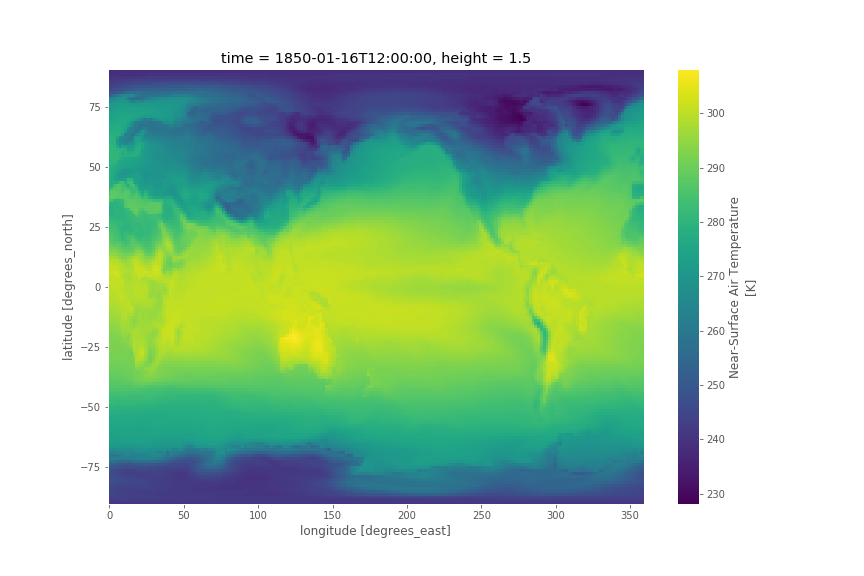
\includegraphics[width=1\textwidth]{gambar1.png}
\end{figure}

Kita juga dapat menerapkan penyeleksian data berantai untuk memvisualisasikan data pada wilayah tertentu pada suatu satuan waktu, seperti pada contoh ini, kita mencoba memvisualisasikan data di Benua Maritim pada bulan Januari 1850:
\begin{lstlisting}[language=Python]
tas.sel(time='1850-01-16T12:00:00',lat=slice(-20,20),lon=slice(90,160)).plot(size=8);
\end{lstlisting}

\begin{figure}[H]
    \centering
    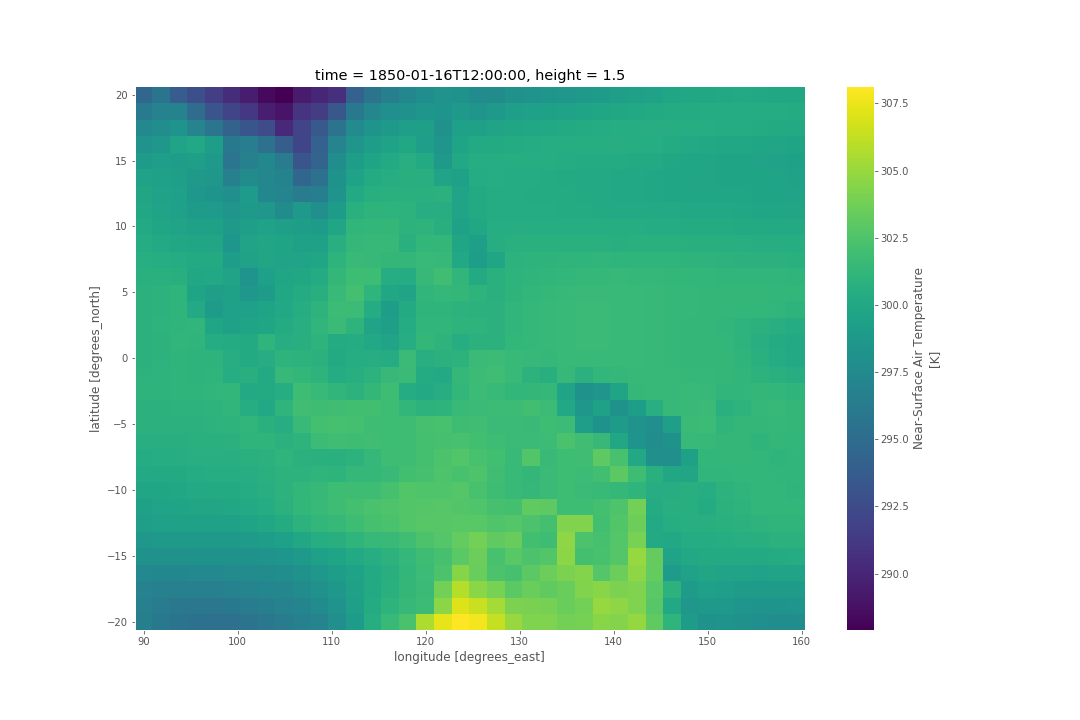
\includegraphics[width=1\textwidth]{gambar2.png}
\end{figure}

Untuk menambahkan peta pada gambar jalankan perintah berikut ini\footnote{Untuk mengetahui secara lebih mendalam tentang pemetaan menggunakan modul cartopy, pembaca disarankan untuk mengunjungi: \url{https://scitools.org.uk/cartopy/docs/latest/}}:

\begin{lstlisting}[language=Python]
import cartopy.crs as ccrs
plt.figure(figsize=(12,8));
data = tas.sel(time='1850-01-16T12:00:00',lat=slice(-20,20),lon=slice(90,160))
ax = plt.axes(projection=ccrs.PlateCarree())
ax.coastlines()
data.plot();
\end{lstlisting}

\begin{figure}[H]
    \centering
    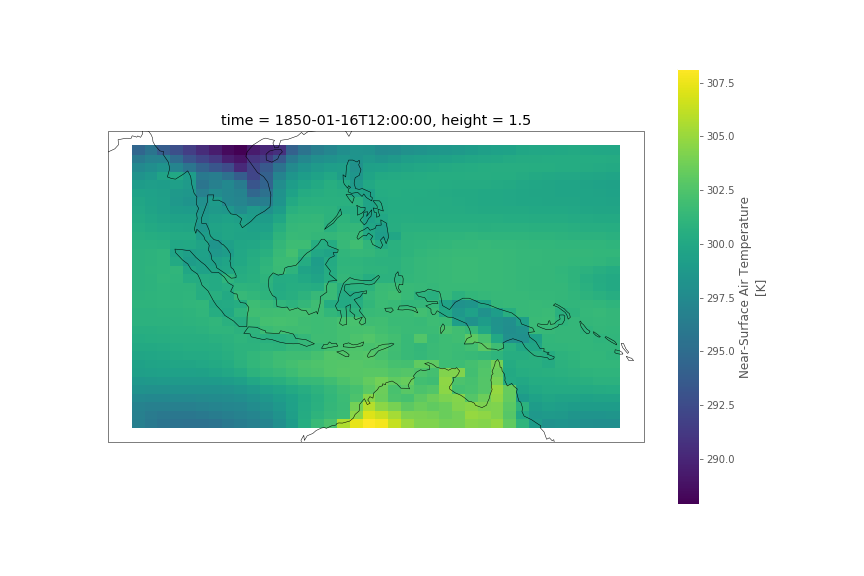
\includegraphics[width=1\textwidth]{gambar3.png}
\end{figure}

\verb|xarray| akan menampilkan data sesuai dengan dimensi data yang kita masukkan ke dalam metode \verb|plot()|. Jika data yang kita masukkan berdimensi banyak, maka metode \verb|plot()| akan menampilkannya sebagai histogram:

\begin{lstlisting}[language=Python]
tas.sel(time=slice('1850-01','1880-12'), lat=slice(-20,20),lon=slice(90,160)).plot(size=6);
\end{lstlisting}

\begin{figure}[H]
    \centering
    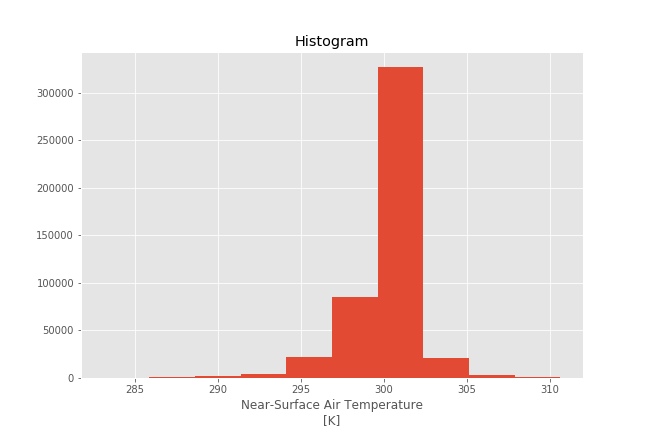
\includegraphics[width=1\textwidth]{gambar4.png}
\end{figure}

Tentunya visualisasi tersebut tidak bermanfaat bagi kita. Namun dengan melakukan reduksi spasial menjadi titik dengan metode \verb|sel()|, kita dapat menampilkan data deret waktu yang (mungkin) dapat kita manfaatkan untuk interpretasi. Pada contoh berikut ini, kita mencoba mengekstraksi temperatur udara dekat permukaan selama 30 tahun (Januari 1850 - Desember 1880) di kota Jakarta:

\begin{lstlisting}[language=Python]
tas.sel(time=slice('1850-01','1880-12')).sel(lat= -6.21462, lon = 106.84513, method='nearest').plot(size=6, marker='o');
\end{lstlisting}
\begin{figure}[H]
    \centering
    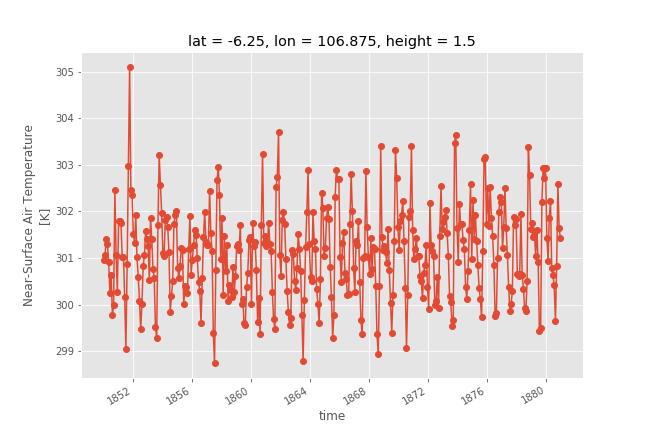
\includegraphics[width=1\textwidth]{gambar5.png}
\end{figure}

Selanjutnya kita akan mencoba membuka data temperatur udara untuk semua level tekanan di model yang sama pada rentang Januari 1850 hingga Desember 1899:

\begin{lstlisting}[language=Python]
ds_temp = xr.open_dataset('ta_Amon_ACCESS1-3_historical_r1i1p1_185001-189912.nc')
ds_temp
\end{lstlisting}
Berikut ini adalah rangkuman dataset-nya:
\begin{lstlisting}[numbers=none]
<xarray.Dataset>
Dimensions:    (bnds: 2, lat: 144, lon: 192, plev: 17, time: 600)
Coordinates:
  * time       (time) datetime64[ns] 1850-01-16T12:00:00 ... 1899-12-16T12:00:00
  * plev       (plev) float64 1e+05 9.25e+04 8.5e+04 7e+04 ... 3e+03 2e+03 1e+03
  * lat        (lat) float64 -89.38 -88.12 -86.88 -85.62 ... 86.88 88.12 89.38
  * lon        (lon) float64 0.9375 2.812 4.688 6.562 ... 355.3 357.2 359.1
Dimensions without coordinates: bnds
Data variables:
    time_bnds  (time, bnds) datetime64[ns] ...
    plev_bnds  (plev, bnds) float64 ...
    lat_bnds   (lat, bnds) float64 ...
    lon_bnds   (lon, bnds) float64 ...
    ta         (time, plev, lat, lon) float32 ...
Attributes:
    institution:            CSIRO (Commonwealth Scientific and Industrial Res...
    institute_id:           CSIRO-BOM
    experiment_id:          historical
    source:                 ACCESS1-3 2011. Atmosphere: AGCM v1.0 (N96 grid-p...
    model_id:               ACCESS1.3
    forcing:                GHG, Oz, SA, Sl, Vl, BC, OC, (GHG = CO2, N2O, CH4...
    parent_experiment_id:   piControl
    parent_experiment_rip:  r1i1p1
    branch_time:            90945.0
    contact:                The ACCESS wiki: http://wiki.csiro.au/confluence/...
    history:                CMIP5 compliant file produced from raw ACCESS mod...
    references:             See http://wiki.csiro.au/confluence/display/ACCES...
    initialization_method:  1
    physics_version:        1
    tracking_id:            eb0cfe7a-9e5d-4ce0-bb72-0c12b500a4d3
    version_number:         v20120413
    product:                output
    experiment:             historical
    frequency:              mon
    creation_date:          2012-03-23T01:31:12Z
    Conventions:            CF-1.4
    project_id:             CMIP5
    table_id:               Table Amon (01 February 2012) 01388cb4507c2f05326...
    title:                  ACCESS1-3 model output prepared for CMIP5 historical
    parent_experiment:      pre-industrial control
    modeling_realm:         atmos
    realization:            1
    cmor_version:           2.8.0
\end{lstlisting}

Selanjutnya kita akan mengekstraksi \verb|DataArray| dari dataset dan menyimpannya dalam variabel \verb|ta|:
\begin{lstlisting}[language=Python]
ta = ds_temp['ta']
ta
\end{lstlisting}

Berikut ini keterangan darii \verb|DataArray| tersebut:
\begin{lstlisting}[numbers=none]
<xarray.DataArray 'ta' (time: 600, plev: 17, lat: 144, lon: 192)>
[282009600 values with dtype=float32]
Coordinates:
  * time     (time) datetime64[ns] 1850-01-16T12:00:00 ... 1899-12-16T12:00:00
  * plev     (plev) float64 1e+05 9.25e+04 8.5e+04 7e+04 ... 3e+03 2e+03 1e+03
  * lat      (lat) float64 -89.38 -88.12 -86.88 -85.62 ... 86.88 88.12 89.38
  * lon      (lon) float64 0.9375 2.812 4.688 6.562 ... 353.4 355.3 357.2 359.1
Attributes:
    standard_name:     air_temperature
    long_name:         Air Temperature
    units:             K
    cell_methods:      time: mean
    cell_measures:     area: areacella
    history:           2012-03-23T01:31:12Z altered by CMOR: replaced missing...
    associated_files:  baseURL: http://cmip-pcmdi.llnl.gov/CMIP5/dataLocation...
\end{lstlisting}

Sebagai penutup bagian ini, kita mencoba memvisualisasikan profil melintang temperatur udara vertikal global dari kutub ke kutub pada garis bujur koordinat Himalaya\footnote{\url{https://www.findlatitudeandlongitude.com/?loc=Himalayas}} di bulan Januari 1850. Kita akan menambahkan argumen \verb|yincrease=False|, karena tekanan berkurang sesuai dengan ketinggian\footnote{\url{http://ww2010.atmos.uiuc.edu/(Gh)/guides/mtr/prs/hght.rxml}}:

\begin{lstlisting}[language=Python]
ta.isel(time=0).sel(lon=82, method='nearest').plot(size=6, yincrease=False);
\end{lstlisting}
Hasilnya adalah:
\begin{figure}[H]
    \centering
    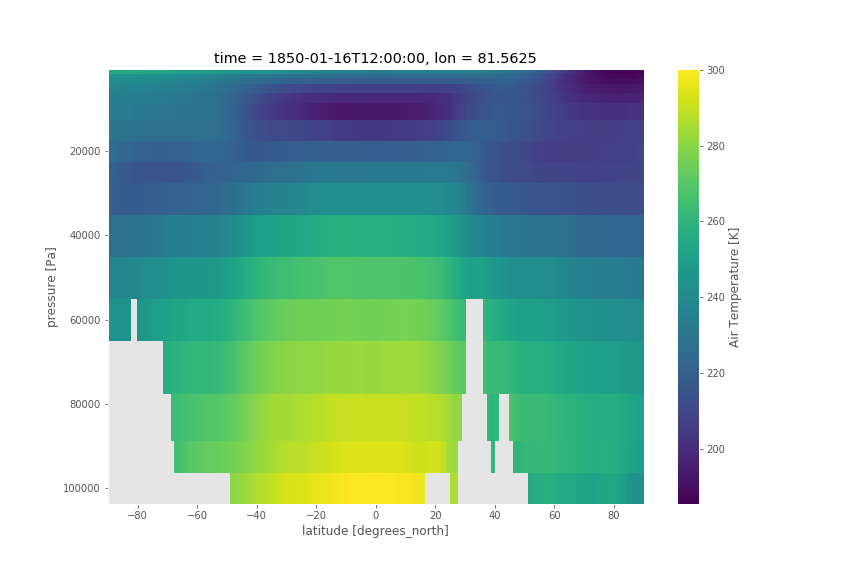
\includegraphics[width=1\textwidth]{gambar6.png}
\end{figure}

\section{Operasi aritmatika sederhana}
\verb|xarray| dibangun di atas pustaka NumPy dan \verb|DataArray| mewarisi sebagian besar metode operasi aritmatika yang dapat dikerjakan pada objek \textit{array}. Pada bagian ini, kita akan membahas beberapa operasi aritmatika sederhana\footnote{Pembahasan tentang metode komputasi lainnya dapat ditemukan di situs: \url{https://xarray.pydata.org/en/stable/computation.html}} pada objek \verb|DataArray| pada data temperatur udara dekat permukaan dalam rentang waktu 1850 - 2005.

Sebagai pengingat, kita akan melihat kembali keterangan pada \verb|DataArray| \verb|tas|:

\begin{lstlisting}[numbers=none]
<xarray.DataArray 'tas' (time: 1872, lat: 145, lon: 192)>
[52116480 values with dtype=float32]
Coordinates:
  * time     (time) datetime64[ns] 1850-01-16T12:00:00 ... 2005-12-16T12:00:00
  * lat      (lat) float64 -90.0 -88.75 -87.5 -86.25 ... 86.25 87.5 88.75 90.0
  * lon      (lon) float64 0.0 1.875 3.75 5.625 7.5 ... 352.5 354.4 356.2 358.1
    height   float64 ...
Attributes:
    standard_name:     air_temperature
    long_name:         Near-Surface Air Temperature
    units:             K
    cell_methods:      time: mean
    cell_measures:     area: areacella
    history:           2012-02-05T23:49:51Z altered by CMOR: Treated scalar d...
    associated_files:  baseURL: http://cmip-pcmdi.llnl.gov/CMIP5/dataLocation...
\end{lstlisting}

Untuk menghitung rata - rata temperatur udara permukaan global pada seluruh periode data, kita dapat menjalankan perintah sederhana berikut ini:
\begin{lstlisting}[language=Python]
tas.mean()
\end{lstlisting}
Hasilnya:
\begin{lstlisting}[numbers=none]
<xarray.DataArray 'tas' ()>
array(277.5926, dtype=float32)
Coordinates:
    height   float64 ...
\end{lstlisting}
\verb|xarray| juga memberikan keleluasaan bagi pengguna untuk menghitung rata - rata berdasarkan dimensi tertentu. Pada contoh ini, kita mencoba untuk menampilkan rata - rata temperatur udara dekat permukaan global sepanjang periode data:

\begin{lstlisting}[language=Python]
plt.figure(figsize=(15,8))
ax = plt.axes(projection=ccrs.PlateCarree())
ax.coastlines()
tas.mean(dim='time').plot();
\end{lstlisting}

\begin{figure}[H]
    \centering
    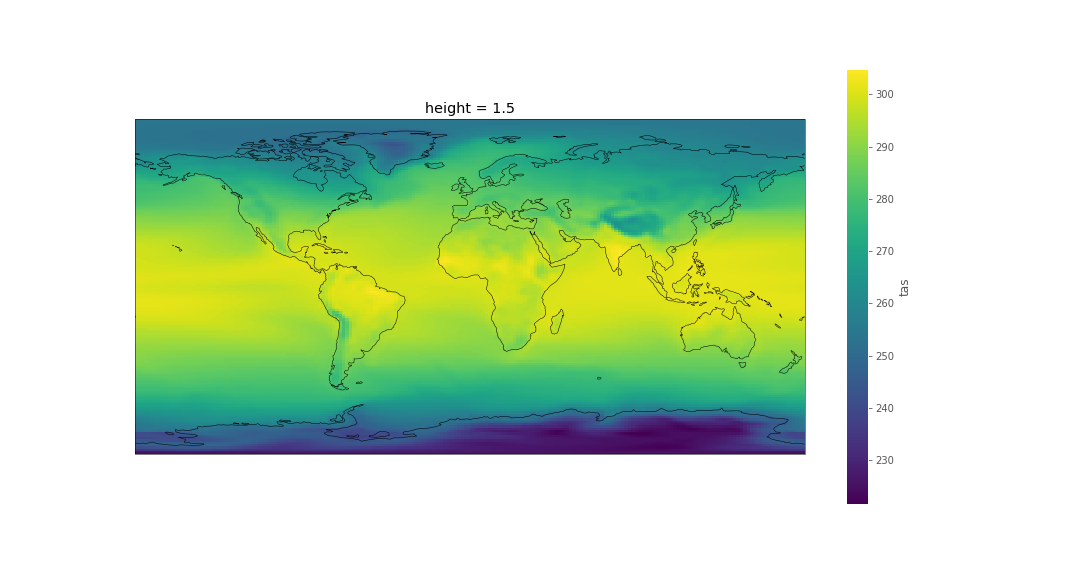
\includegraphics[width=1\textwidth]{gambar7.png}
\end{figure}

Di bidang keilmuan klimatologi, adalah hal umum untuk menghitung rata - rata data iklim selama tiga puluh tahun\footnote{World Meteorological Organization. 2017. WMO Guidelines on the calculation of climate normals. Geneva: World Meteorological Organization.}. Hal ini dimungkinkan dengan menggunakan metode \verb|sel()| pada \verb|DataArray|:

\begin{lstlisting}[language=Python]
tas_clim = tas.sel(time=slice('1961-01','1990-12')).mean(dim='time')
plt.figure(figsize=(15,8))
ax = plt.axes(projection=ccrs.PlateCarree())
ax.coastlines()
tas_clim.plot();
\end{lstlisting}

\begin{figure}[H]
    \centering
    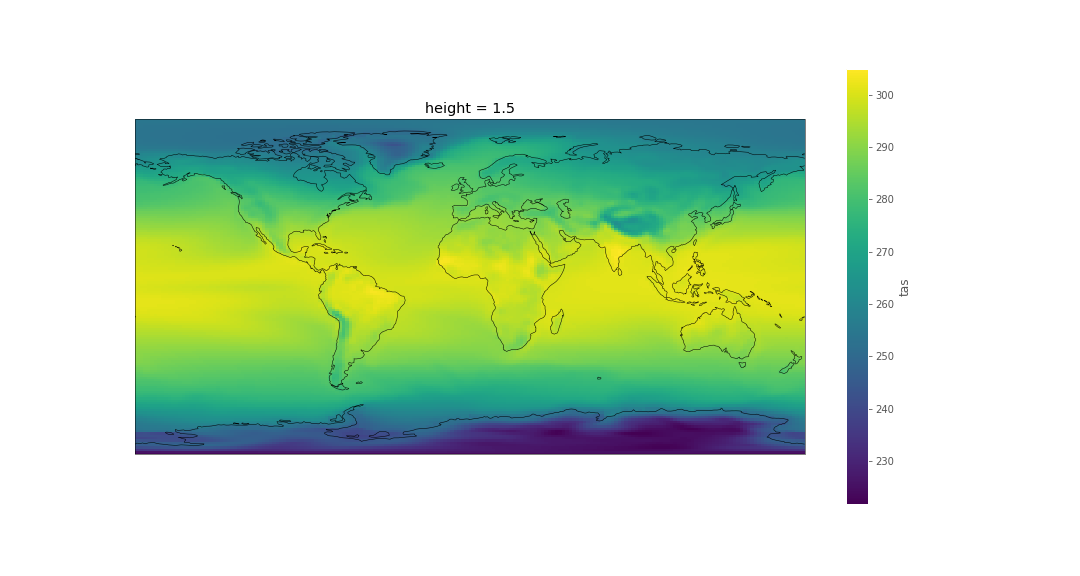
\includegraphics[width=1\textwidth]{gambar8.png}
\end{figure}

Kita juga dapat menghitung anomali iklim sepanjang periode data terhadap acuan iklim modern\footnote{\url{http://www.bom.gov.au/climate/glossary/anomaly.shtml}} dengan cara sebagai berikut:
\begin{lstlisting}[language=Python]
tas_anom = (tas - tas_clim)
tas_anom
\end{lstlisting}
\verb|xarray| akan secara otomatis memeriksa koordinat yang memiliki penamaan yang sama, sehingga dapat melakukan operasi hanya pada dimensi waktu. Berikut ini hasil perhitungannya:
\begin{lstlisting}[numbers=none]
<xarray.DataArray 'tas' (time: 1872, lat: 145, lon: 192)>
array([[[ 1.72964630e+01,  1.72964630e+01,  1.72964630e+01, ...,
          1.73007202e+01,  1.73007202e+01,  1.73007202e+01],
        [ 1.56811066e+01,  1.57091217e+01,  1.57379303e+01, ...,
          1.55756683e+01,  1.56139221e+01,  1.56476593e+01],
        [ 1.54892426e+01,  1.55479279e+01,  1.55988159e+01, ...,
          1.52837067e+01,  1.53598328e+01,  1.54254761e+01],
        ...,
        [-1.55937042e+01, -1.55449371e+01, -1.54929504e+01, ...,
         -1.57009735e+01, -1.56634369e+01, -1.56276245e+01],
        [-1.58852386e+01, -1.58901062e+01, -1.58975525e+01, ...,
         -1.58176727e+01, -1.58402710e+01, -1.58671875e+01],
        [-1.57813721e+01, -1.57813721e+01, -1.57813721e+01, ...,
         -1.57813721e+01, -1.57813721e+01, -1.57813721e+01]],

       [[ 9.73437500e+00,  9.73437500e+00,  9.73437500e+00, ...,
          9.73960876e+00,  9.73960876e+00,  9.73960876e+00],
        [ 8.44528198e+00,  8.46022034e+00,  8.47381592e+00, ...,
          8.40753174e+00,  8.41888428e+00,  8.43382263e+00],
        [ 7.64672852e+00,  7.65853882e+00,  7.67440796e+00, ...,
          7.63131714e+00,  7.63415527e+00,  7.63662720e+00],
        ...,
        [-1.71459198e+01, -1.72234039e+01, -1.72892914e+01, ...,
         -1.69746704e+01, -1.70062408e+01, -1.70744324e+01],
        [-1.81874695e+01, -1.81761627e+01, -1.81784058e+01, ...,
         -1.82436676e+01, -1.82273102e+01, -1.82099915e+01],
        [-1.98102112e+01, -1.98102112e+01, -1.98102112e+01, ...,
         -1.98102112e+01, -1.98102112e+01, -1.98102112e+01]],

       [[-2.81030273e+00, -2.81030273e+00, -2.81030273e+00, ...,
         -2.80503845e+00, -2.80503845e+00, -2.80503845e+00],
        [-1.62951660e+00, -1.62695312e+00, -1.62425232e+00, ...,
         -1.65043640e+00, -1.64112854e+00, -1.63494873e+00],
        [-1.67668152e+00, -1.67411804e+00, -1.66809082e+00, ...,
         -1.67835999e+00, -1.67826843e+00, -1.67810059e+00],
        ...,
        [-1.34598236e+01, -1.34111786e+01, -1.33634644e+01, ...,
         -1.35620270e+01, -1.35296478e+01, -1.35029449e+01],
        [-1.35711517e+01, -1.35783844e+01, -1.35777740e+01, ...,
         -1.35734100e+01, -1.35773773e+01, -1.35726013e+01],
        [-1.34223175e+01, -1.34223175e+01, -1.34223175e+01, ...,
         -1.34223175e+01, -1.34223175e+01, -1.34223175e+01]],

       ...,

       [[-2.85758972e+00, -2.85758972e+00, -2.85758972e+00, ...,
         -2.85961914e+00, -2.85961914e+00, -2.85961914e+00],
        [-1.19322205e+00, -1.19934082e+00, -1.20622253e+00, ...,
         -1.17553711e+00, -1.17979431e+00, -1.18693542e+00],
        [-1.94763184e-01, -2.35382080e-01, -2.77450562e-01, ...,
         -9.29870605e-02, -1.22222900e-01, -1.56570435e-01],
        ...,
        [-8.16192627e-02,  5.23529053e-02,  1.90399170e-01, ...,
         -4.29809570e-01, -3.15368652e-01, -1.99523926e-01],
        [ 7.58972168e-02,  1.48269653e-01,  2.37060547e-01, ...,
         -1.44454956e-01, -8.88519287e-02, -7.62939453e-04],
        [ 3.66500854e-01,  3.66500854e-01,  3.66500854e-01, ...,
          3.66500854e-01,  3.66500854e-01,  3.66500854e-01]],

       [[ 1.47180634e+01,  1.47180634e+01,  1.47180634e+01, ...,
          1.47147980e+01,  1.47147980e+01,  1.47147980e+01],
        [ 1.32177277e+01,  1.32196655e+01,  1.32233124e+01, ...,
          1.32041931e+01,  1.32099152e+01,  1.32117767e+01],
        [ 1.31987610e+01,  1.32250366e+01,  1.32500153e+01, ...,
          1.31194611e+01,  1.31459351e+01,  1.31743011e+01],
        ...,
        [ 2.49589539e+00,  2.51516724e+00,  2.56269836e+00, ...,
          2.37658691e+00,  2.42333984e+00,  2.45704651e+00],
        [ 2.15078735e+00,  2.17623901e+00,  2.18557739e+00, ...,
          2.09861755e+00,  2.11506653e+00,  2.13304138e+00],
        [ 1.23558044e+00,  1.23558044e+00,  1.23558044e+00, ...,
          1.23558044e+00,  1.23558044e+00,  1.23558044e+00]],

       [[ 2.29509125e+01,  2.29509125e+01,  2.29509125e+01, ...,
          2.29463043e+01,  2.29463043e+01,  2.29463043e+01],
        [ 2.06225433e+01,  2.06300201e+01,  2.06369019e+01, ...,
          2.05933228e+01,  2.06056824e+01,  2.06126709e+01],
        [ 2.04603577e+01,  2.04730682e+01,  2.04817047e+01, ...,
          2.04244690e+01,  2.04382019e+01,  2.04499969e+01],
        ...,
        [-7.15808105e+00, -7.11807251e+00, -7.10719299e+00, ...,
         -7.37442017e+00, -7.27648926e+00, -7.20214844e+00],
        [-7.76913452e+00, -7.73861694e+00, -7.71789551e+00, ...,
         -7.87310791e+00, -7.83821106e+00, -7.79762268e+00],
        [-7.95593262e+00, -7.95593262e+00, -7.95593262e+00, ...,
         -7.95593262e+00, -7.95593262e+00, -7.95593262e+00]]],
      dtype=float32)
Coordinates:
  * time     (time) datetime64[ns] 1850-01-16T12:00:00 ... 2005-12-16T12:00:00
  * lat      (lat) float64 -90.0 -88.75 -87.5 -86.25 ... 86.25 87.5 88.75 90.0
  * lon      (lon) float64 0.0 1.875 3.75 5.625 7.5 ... 352.5 354.4 356.2 358.1
    height   float64 1.5
\end{lstlisting}

Kita juga dapat mengekstraksi rata - rata anomali iklim global pada periode waktu tertentu dengan menggunakan perintah sebagai berikut:
\begin{lstlisting}
tas_anom.sel(time=slice('1850-01', '1879-12')).mean(dim=('lat','lon')).plot(size=6);
\end{lstlisting}

\begin{figure}[H]
    \centering
    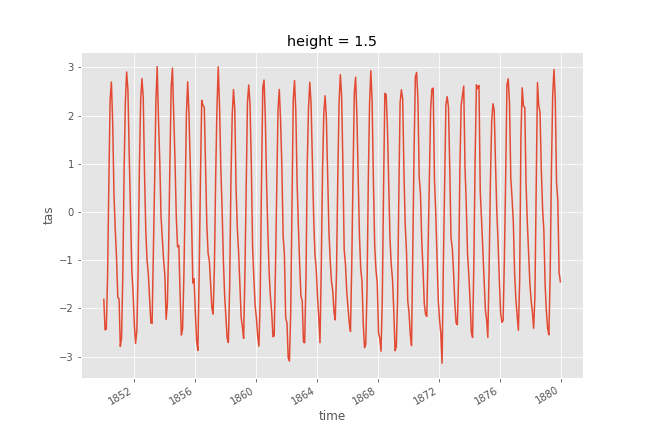
\includegraphics[width=1\textwidth]{gambar9.png}
\end{figure}

\section{Pengelompokan dan pensampelan ulang data}

\verb|xarray| dibangun di atas pustaka pandas yang terkenal dengan keunggulannya untuk menganalisis data deret waktu (\textit{time-series}) pada tipe data tabular dan objek \verb|datetime|\footnote{\url{https://kite.com/blog/python/pandas-time-series-analysis/}}. Oleh karena itu, \verb|xarray| juga mewarisi kelebihan - kelebihan tersebut\footnote{Untuk lebih jelasnya pembaca disarankan untuk mengunjungi situs \url{https://xarray.pydata.org/en/stable/groupby.html} dan \url{https://xarray.pydata.org/en/stable/time-series.html}}.

Untuk mengawali pembahasan, saya akan mencoba menampilkan kembali hasil perhitungan anomali temperatur udara dekat permukaan yang telah kita lakukan sebelumnya:

\begin{lstlisting}[numbers=none]
<xarray.DataArray 'tas' (time: 1872, lat: 145, lon: 192)>
array([[[ 1.72964630e+01,  1.72964630e+01,  1.72964630e+01, ...,
          1.73007202e+01,  1.73007202e+01,  1.73007202e+01],
        [ 1.56811066e+01,  1.57091217e+01,  1.57379303e+01, ...,
          1.55756683e+01,  1.56139221e+01,  1.56476593e+01],
        [ 1.54892426e+01,  1.55479279e+01,  1.55988159e+01, ...,
          1.52837067e+01,  1.53598328e+01,  1.54254761e+01],
        ...,
        [-1.55937042e+01, -1.55449371e+01, -1.54929504e+01, ...,
         -1.57009735e+01, -1.56634369e+01, -1.56276245e+01],
        [-1.58852386e+01, -1.58901062e+01, -1.58975525e+01, ...,
         -1.58176727e+01, -1.58402710e+01, -1.58671875e+01],
        [-1.57813721e+01, -1.57813721e+01, -1.57813721e+01, ...,
         -1.57813721e+01, -1.57813721e+01, -1.57813721e+01]],

       [[ 9.73437500e+00,  9.73437500e+00,  9.73437500e+00, ...,
          9.73960876e+00,  9.73960876e+00,  9.73960876e+00],
        [ 8.44528198e+00,  8.46022034e+00,  8.47381592e+00, ...,
          8.40753174e+00,  8.41888428e+00,  8.43382263e+00],
        [ 7.64672852e+00,  7.65853882e+00,  7.67440796e+00, ...,
          7.63131714e+00,  7.63415527e+00,  7.63662720e+00],
        ...,
        [-1.71459198e+01, -1.72234039e+01, -1.72892914e+01, ...,
         -1.69746704e+01, -1.70062408e+01, -1.70744324e+01],
        [-1.81874695e+01, -1.81761627e+01, -1.81784058e+01, ...,
         -1.82436676e+01, -1.82273102e+01, -1.82099915e+01],
        [-1.98102112e+01, -1.98102112e+01, -1.98102112e+01, ...,
         -1.98102112e+01, -1.98102112e+01, -1.98102112e+01]],

       [[-2.81030273e+00, -2.81030273e+00, -2.81030273e+00, ...,
         -2.80503845e+00, -2.80503845e+00, -2.80503845e+00],
        [-1.62951660e+00, -1.62695312e+00, -1.62425232e+00, ...,
         -1.65043640e+00, -1.64112854e+00, -1.63494873e+00],
        [-1.67668152e+00, -1.67411804e+00, -1.66809082e+00, ...,
         -1.67835999e+00, -1.67826843e+00, -1.67810059e+00],
        ...,
        [-1.34598236e+01, -1.34111786e+01, -1.33634644e+01, ...,
         -1.35620270e+01, -1.35296478e+01, -1.35029449e+01],
        [-1.35711517e+01, -1.35783844e+01, -1.35777740e+01, ...,
         -1.35734100e+01, -1.35773773e+01, -1.35726013e+01],
        [-1.34223175e+01, -1.34223175e+01, -1.34223175e+01, ...,
         -1.34223175e+01, -1.34223175e+01, -1.34223175e+01]],

       ...,

       [[-2.85758972e+00, -2.85758972e+00, -2.85758972e+00, ...,
         -2.85961914e+00, -2.85961914e+00, -2.85961914e+00],
        [-1.19322205e+00, -1.19934082e+00, -1.20622253e+00, ...,
         -1.17553711e+00, -1.17979431e+00, -1.18693542e+00],
        [-1.94763184e-01, -2.35382080e-01, -2.77450562e-01, ...,
         -9.29870605e-02, -1.22222900e-01, -1.56570435e-01],
        ...,
        [-8.16192627e-02,  5.23529053e-02,  1.90399170e-01, ...,
         -4.29809570e-01, -3.15368652e-01, -1.99523926e-01],
        [ 7.58972168e-02,  1.48269653e-01,  2.37060547e-01, ...,
         -1.44454956e-01, -8.88519287e-02, -7.62939453e-04],
        [ 3.66500854e-01,  3.66500854e-01,  3.66500854e-01, ...,
          3.66500854e-01,  3.66500854e-01,  3.66500854e-01]],

       [[ 1.47180634e+01,  1.47180634e+01,  1.47180634e+01, ...,
          1.47147980e+01,  1.47147980e+01,  1.47147980e+01],
        [ 1.32177277e+01,  1.32196655e+01,  1.32233124e+01, ...,
          1.32041931e+01,  1.32099152e+01,  1.32117767e+01],
        [ 1.31987610e+01,  1.32250366e+01,  1.32500153e+01, ...,
          1.31194611e+01,  1.31459351e+01,  1.31743011e+01],
        ...,
        [ 2.49589539e+00,  2.51516724e+00,  2.56269836e+00, ...,
          2.37658691e+00,  2.42333984e+00,  2.45704651e+00],
        [ 2.15078735e+00,  2.17623901e+00,  2.18557739e+00, ...,
          2.09861755e+00,  2.11506653e+00,  2.13304138e+00],
        [ 1.23558044e+00,  1.23558044e+00,  1.23558044e+00, ...,
          1.23558044e+00,  1.23558044e+00,  1.23558044e+00]],

       [[ 2.29509125e+01,  2.29509125e+01,  2.29509125e+01, ...,
          2.29463043e+01,  2.29463043e+01,  2.29463043e+01],
        [ 2.06225433e+01,  2.06300201e+01,  2.06369019e+01, ...,
          2.05933228e+01,  2.06056824e+01,  2.06126709e+01],
        [ 2.04603577e+01,  2.04730682e+01,  2.04817047e+01, ...,
          2.04244690e+01,  2.04382019e+01,  2.04499969e+01],
        ...,
        [-7.15808105e+00, -7.11807251e+00, -7.10719299e+00, ...,
         -7.37442017e+00, -7.27648926e+00, -7.20214844e+00],
        [-7.76913452e+00, -7.73861694e+00, -7.71789551e+00, ...,
         -7.87310791e+00, -7.83821106e+00, -7.79762268e+00],
        [-7.95593262e+00, -7.95593262e+00, -7.95593262e+00, ...,
         -7.95593262e+00, -7.95593262e+00, -7.95593262e+00]]],
      dtype=float32)
Coordinates:
  * time     (time) datetime64[ns] 1850-01-16T12:00:00 ... 2005-12-16T12:00:00
  * lat      (lat) float64 -90.0 -88.75 -87.5 -86.25 ... 86.25 87.5 88.75 90.0
  * lon      (lon) float64 0.0 1.875 3.75 5.625 7.5 ... 352.5 354.4 356.2 358.1
    height   float64 1.5
\end{lstlisting}

Selanjutnya, kita mencoba memvisualisasikan rata - rata anomali temperatur udara dekat permukaan global dari Januari 1961, hingga akhir periode data:

\begin{lstlisting}[language=Python]
tas_anom.sel(time=slice('1961-01',None)).mean(dim=('lat','lon')).plot(size=8);
\end{lstlisting}

\begin{figure}[H]
    \centering
    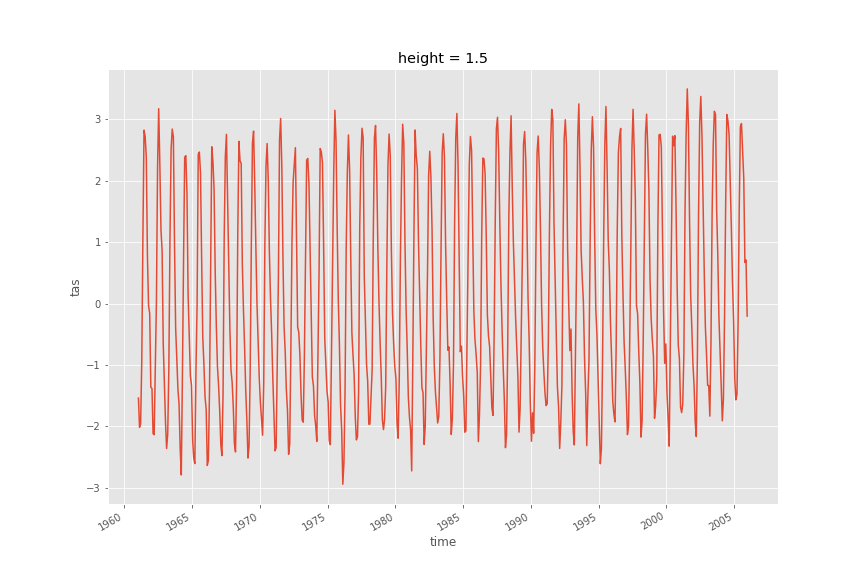
\includegraphics[width=1\textwidth]{gambar10.png}
\end{figure}

Untuk melihat tren pemanasan global, kita dapat melakukan pensamplingan (\textit{resampling}) data untuk frekuensi tahunan. Metode yang digunakan pada \verb|xarray| untuk menerapkan teknik ini adalah \verb|resampling()|. Berikut ini contoh penggunaanya untuk \textit{resampling} anomali rata - rata tahunan (dengan menggunakan metode \verb|mean()|):

\begin{lstlisting}[language=Python]
tas_anom_tahunan = tas_anom.sel(time=slice('1961-01',None)).resample(time='Y').mean(dim='time')
tas_anom_tahunan.dims, tas_anom_tahunan.shape
\end{lstlisting}
Berikut ini dimensi dan ukuran data \textit{resampling} tahunan tersebut:
\begin{lstlisting}[numbers=none]
(('time', 'lat', 'lon'), (45, 145, 192))
\end{lstlisting}
Nampak bahwa ukuran pada dimensi waktu telah tereduksi menjadi \verb|46|.

Untuk melihat tren pemanasan global secara lebih jelas, kita dapat memvisualisasikan data anomali tahunan secara global dengan menggunakan perintah sebagai berikut:

\begin{lstlisting}[language=Python]
tas_anom_tahunan.mean(dim=('lat','lon')).plot(size=8);
\end{lstlisting}

\begin{figure}[H]
    \centering
    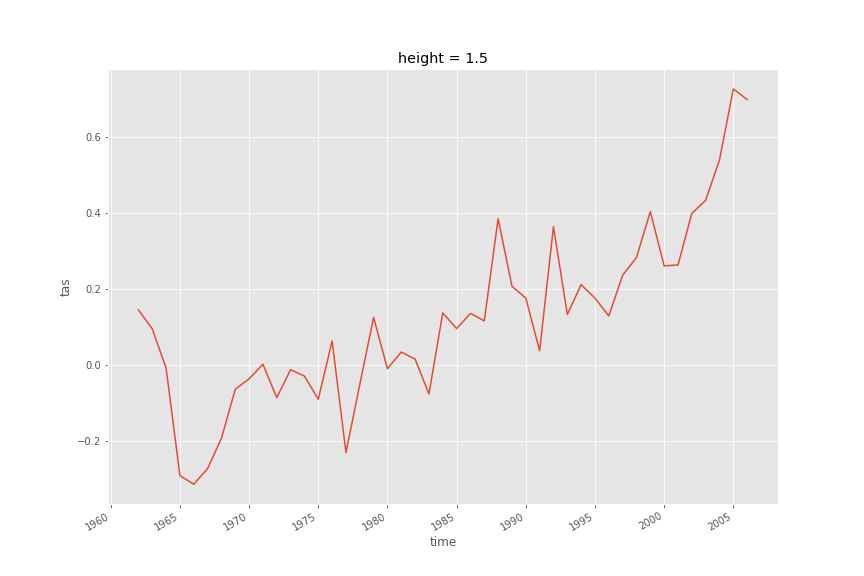
\includegraphics[width=1\textwidth]{gambar11.png}
\end{figure}

Karena data \verb|tas_anom_tahunan| masih mempunyai dimensi spasial, kita dapat menggunakan metode \verb|sel()| untuk menampilkan data anomali tahunan berdasarkan belahan bumi yang berbeda:

\begin{lstlisting}[language=Python]
ax = plt.axes()
ax.figure.set_size_inches(12, 8)
tas_anom_tahunan.mean(dim=('lat','lon')).plot(ax=ax, label='Global');
tas_anom_tahunan.sel(lat=slice(0,None)).mean(dim=('lat','lon')).plot(ax=ax, label='Belahan Bumi Utara');
tas_anom_tahunan.sel(lat=slice(None,0)).mean(dim=('lat','lon')).plot(ax=ax, label='Belahan Bumi Selatan');
plt.title('Anomali temperatur berdasarkan klimatologi 1961-2005')
plt.legend();
\end{lstlisting}

\begin{figure}[H]
    \centering
    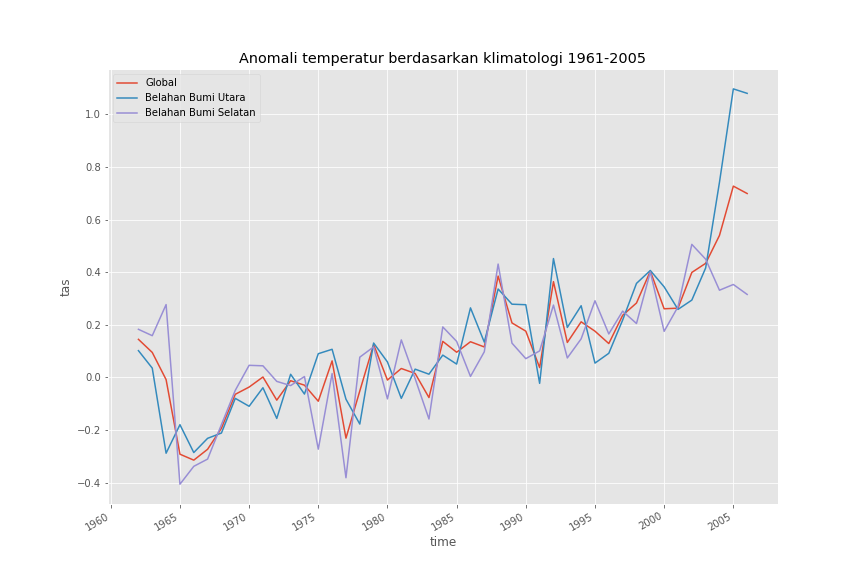
\includegraphics[width=1\textwidth]{gambar12.png}
\end{figure}

Melalui grafik tersebut kita dapat menyimpulkan secara kualitatif bahwa pada sebagian besar periode data, tren pada kedua belahan bumi tersebut hampir seragam, namun pada tahun - tahun terakhir anomali temperatur di belahan bumi utara menunjukkan peningkatan yang cukup tajam.

Kita dapat mengelompokan data berdasarkan garis lintang-nya melalui metode \verb|groupby_bins()|. Untuk memahami prinsip kerja metode ini, kita akan mencoba menampilkan \textit{tuple} yang memuat interval lintang, dimensi, dan ukuran objek \verb|DataArray| yang dihasilkan melalui metode \verb|groupby_bins()| dengan membagi garis lintang bumi menjadi lima bagian:

\begin{lstlisting}[language=Python]
for i, d in tas_anom_tahunan.groupby_bins('lat', bins=5):
    print(i, d.dims, d.shape)
\end{lstlisting}

Hasilnya adalah:
\begin{lstlisting}[numbers=none]
(-90.18, -54.0] ('time', 'lat', 'lon') (45, 29, 192)
(-54.0, -18.0] ('time', 'lat', 'lon') (45, 29, 192)
(-18.0, 18.0] ('time', 'lat', 'lon') (45, 29, 192)
(18.0, 54.0] ('time', 'lat', 'lon') (45, 29, 192)
(54.0, 90.0] ('time', 'lat', 'lon') (45, 29, 192)
\end{lstlisting}

Berikut ini perintah yang kita gunakan untuk memvisualisasikan anomali rata - rata temperatur udara dekat permukaan bulanan selama kurun waktu Januari 1961 hingga Desember 2005 melalui skema pembagian lima zona lintang:

\begin{lstlisting}[language=Python]
tas_anom_yearly.groupby_bins('lat', bins=10).mean(dim=('lat','lon')).plot(x='time',hue='lat_bins',size=8)
\end{lstlisting}

\begin{figure}[H]
    \centering
    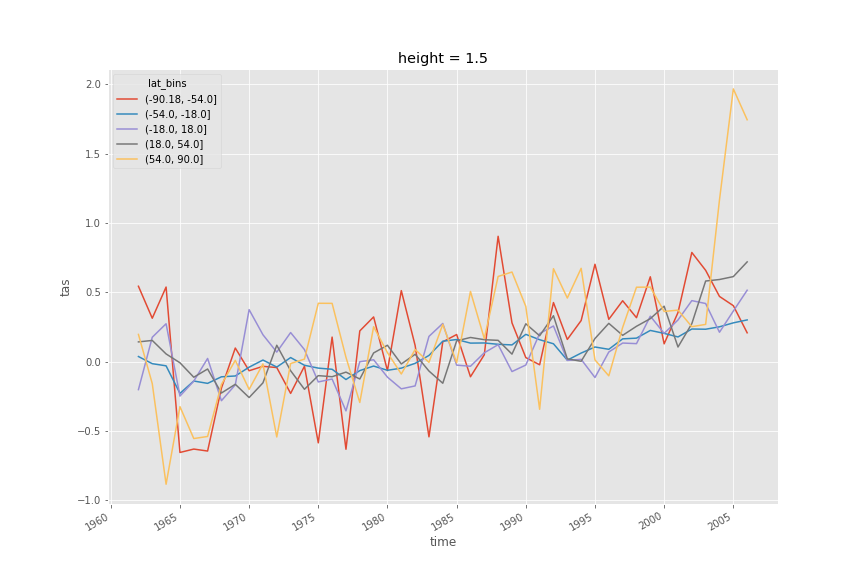
\includegraphics[width=1\textwidth]{gambar13.png}
\end{figure}

\verb|xarray| mempunyai koordinat waktu virtual yang sangat bermanfaat bagi penelitian geosains, yakni \verb|time.season|. Oleh karena itu, kita dapat mengelompokan data menurut rata - rata musimannya dengan cara yang sangat mudah. Berikut ini adalah contoh visual sederhana nilai rata - rata temperatur udara dekat permukaan musiman:

\begin{lstlisting}[language=Python]
tas.groupby('time.season').mean(dim='time').plot(col='season', col_wrap=2);
\end{lstlisting}

\begin{figure}[H]
    \centering
    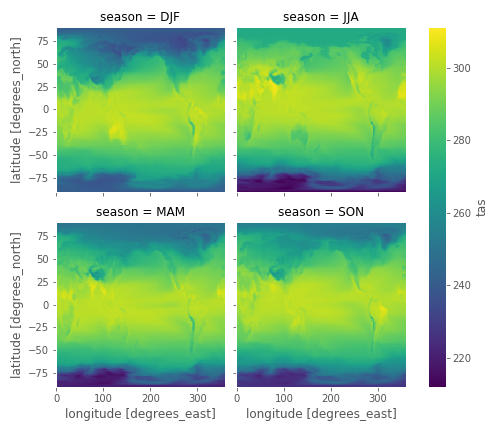
\includegraphics[width=1\textwidth]{gambar14.png}
\end{figure}

\section{\textit{Masking}}
\verb|xarray| menyediakan metode \verb|where()| yang dapat digunakan untuk memfilter \verb|DataArray|. Kita akan menggunakan \verb|DataArray| \verb|tas| pada bagian ini.

Kita dapat melakukan operasi \verb|masking| suatu \verb|DataArray| terhadap dirinya sendiri untuk rentang nilai tertentu. Misalkan pada contoh ini, kita mencoba untuk hanya menampilkan data temperatur udara permukaan pada Desember 2005 pada rentang nilai 273 K hingga 300 K:

\begin{lstlisting}[language=Python]
tasDes2005 = tas.isel(time=-1)
tasDes2005.where(tasDes2005>273).where(tasDes2005<300).plot(size=8);
\end{lstlisting}

\begin{figure}[H]
    \centering
    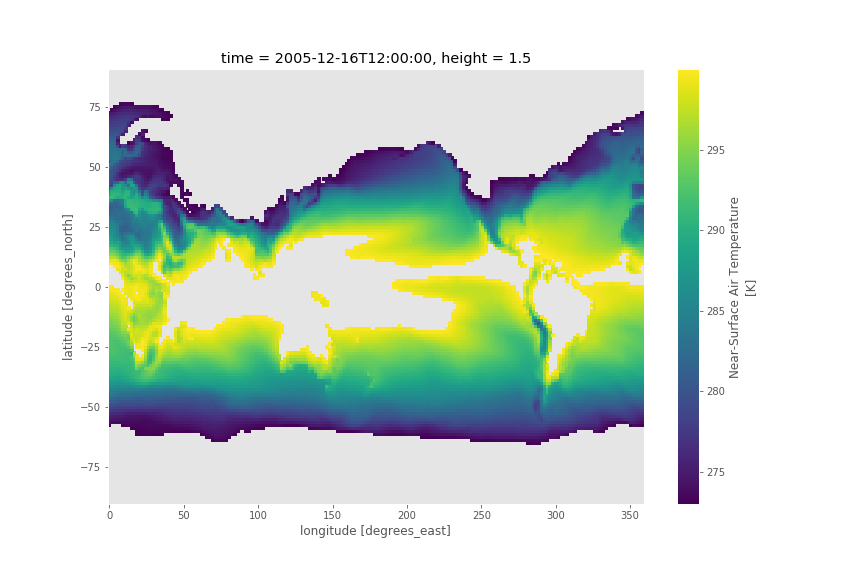
\includegraphics[width=1\textwidth]{gambar15.png}
\end{figure}

Kita juga dapat melakukan operasi \textit{masking} untuk \verb|DataArray| yang sama untuk periode waktu yang berbeda, seperti pada contoh ini, kita hendak menampilkan wilayah dengan temperatur udara permukaan di bulan Desember 2005 pada rentang nilai 273 K hingga 300 K, pada bulan Januari 1850 dengan menambahkan kriteria waktu melalui metode \verb|isel()|:

\begin{lstlisting}[language=Python]
tas.where(tasDes2005>273).where(tasDes2005<300).isel(time=0).plot(size=8);
\end{lstlisting}

\begin{figure}[H]
    \centering
    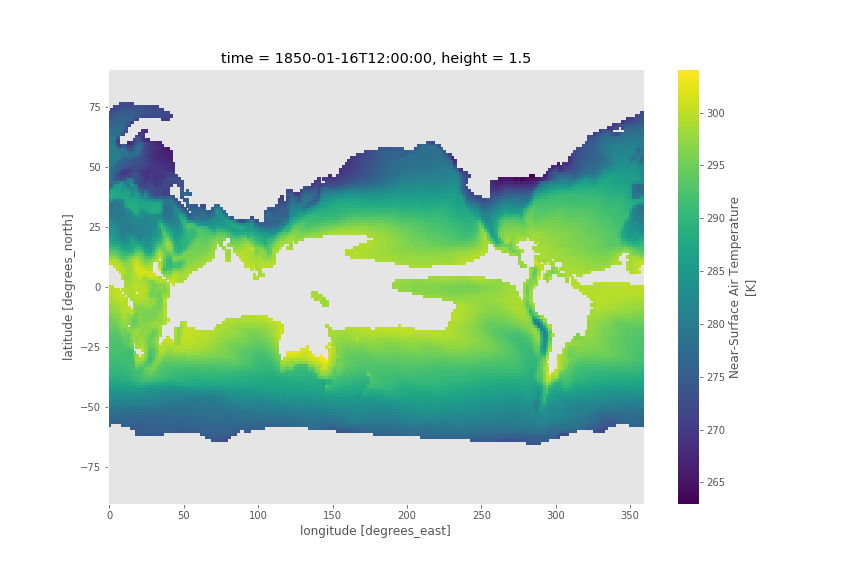
\includegraphics[width=1\textwidth]{gambar16.png}
\end{figure}

Meskipun, pada hakikatnya tidak begitu bermanfaat, namun \verb|xarray| juga dapat menggunakan koordinat lintang dan/atau bujur sebagai \textit{mask}. Perhatikanlah contoh berikut ini, di mana saya akan menunjukkan bahwa kita dapat melakukan \textit{masking} dengan beberapa parameter menggunakan dua buah argumen pada metode \verb|where()|:

\begin{lstlisting}[language=Python]
fig, axes = plt.subplots(ncols=2,figsize=(12,6))
tasDes2005.where(tasDes2005.lat<20, 270).plot(ax=axes[0]);
tasDes2005.where(tasDes2005.lat<25, tas.isel(time=2)).plot(ax=axes[1]);
\end{lstlisting}

\begin{figure}[H]
    \centering
    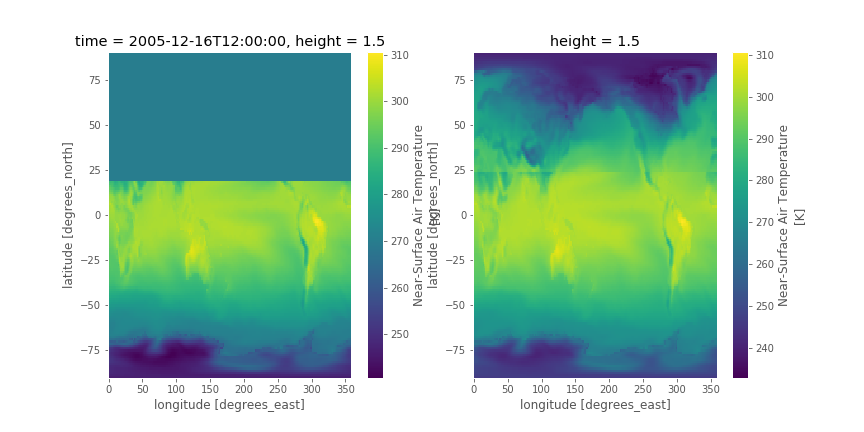
\includegraphics[width=1\textwidth]{gambar17.png}
\end{figure}

Selain itu, kita juga dapat melakukan operasi \textit{masking} dengan menggunakan data NetCDF yang berbeda asalkan memiliki ukuran dan koordinat referensi yang sama. Kita akan menggunakan data \verb|sftlf_fx| (fluks fraksinasi daratan) dari eksperimen model yang sama sebagai \textit{mask} bagi data temperatur udara dekat permukaan pada Januari 1850, guna mendapatkan data temperatur daratan, karena nilai \verb|sftlf_fx| pada laut bernilai nol\footnote{\url{https://carpentrieslab.github.io/python-aos-lesson/07-vectorisation/index.html}}:

\begin{lstlisting}[language=Python]
plt.figure(figsize=(15,8));
sftlf = xr.open_dataset('sftlf_fx_ACCESS1-3_historical_r0i0p0.nc')['sftlf']
ax = plt.axes(projection=ccrs.PlateCarree())
ax.coastlines()
tas.isel(time=0).where(sftlf>0).plot();
\end{lstlisting}

\begin{figure}[H]
    \centering
    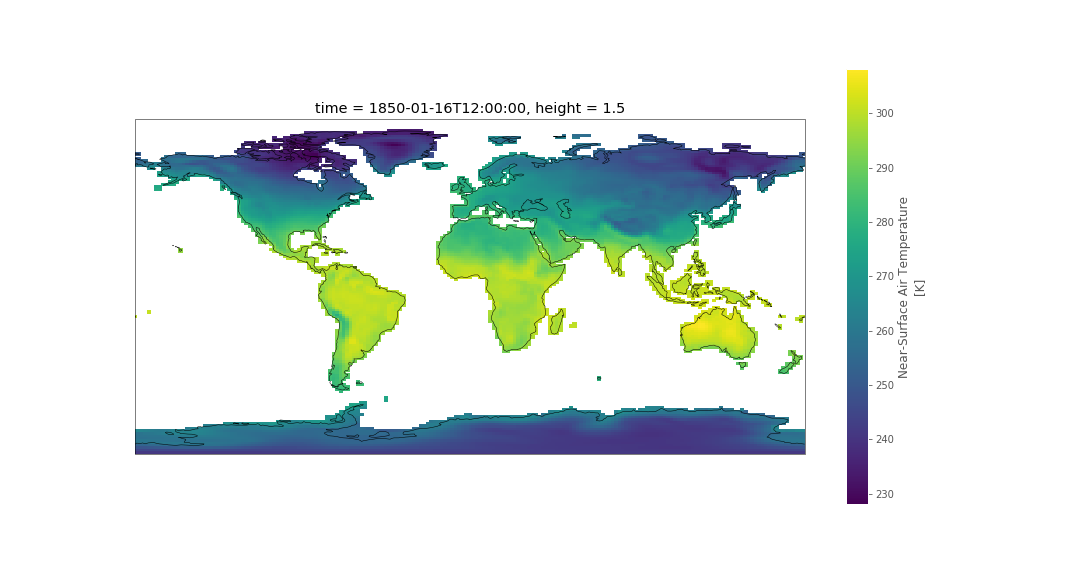
\includegraphics[width=1.2\textwidth]{gambar18.png}
\end{figure}

Dengan melakukan pemisahan antara temperatur udara laut dan daratan, kita dapat menghitung anomali temperatur udara dekat permukaan global secara terpisah:

\begin{lstlisting}[language=Python]
axes = plt.axes()
axes.figure.set_size_inches(12, 8)
tas_anom_tahunan.where(sftlf > 0).mean(dim=('lat','lon')).plot(label='Daratan', ax=axes);
tas_anom_tahunan.where(sftlf ==0).mean(dim=('lat','lon')).plot(label='Laut', ax=axes);
tas_anom_tahunan.mean(dim=('lat','lon')).plot(label='Global', ax=axes);
plt.legend();
\end{lstlisting}

\begin{figure}[H]
    \centering
    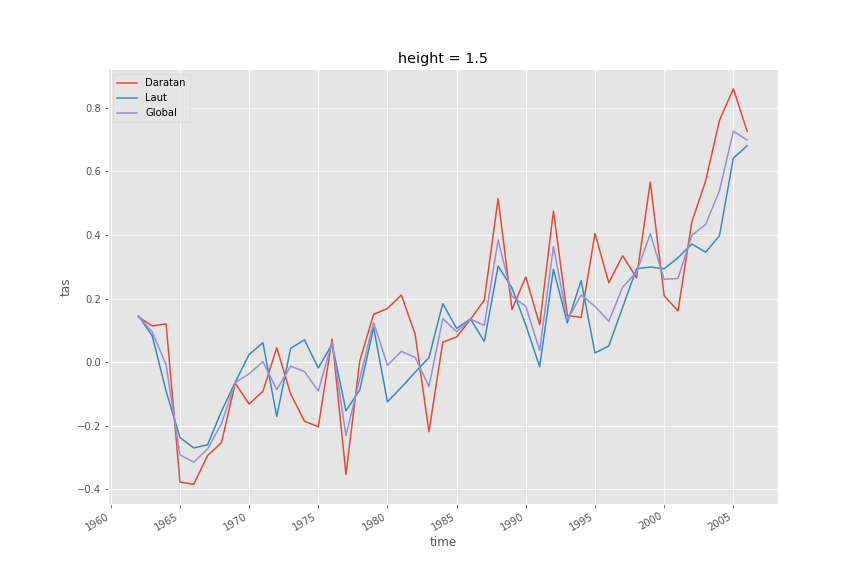
\includegraphics[width=1\textwidth]{gambar19.png}
\end{figure}

\section{Membuka dataset dalam jumlah banyak}
Dalam banyak kasus, luaran model iklim global terkadang terbagi menjadi beberapa file berdasarkan periode waktu. Hal ini menyultikan kita dalam menggabungkan dataset tersebut untuk dijadikan bahan analisis. \verb|xarray| menawarkan kemudahan untuk menggabungkan beberapa dataset tersebut dengan menggunakan fungsi \verb|open_mfdataset()|. Kita akan mengawali pembahasan ini dengan menggabungkan data temperatur udara dekat permukaan harian dari Januari 1850 hingga Desember 1924 yang terbagi ke dalam tiga buah file terpisah:

\begin{lstlisting}[language=Python]
lds = ['tas_day_ACCESS1-3_historical_r1i1p1_18500101-18741231.nc',
       'tas_day_ACCESS1-3_historical_r1i1p1_18750101-18991231.nc',
      'tas_day_ACCESS1-3_historical_r1i1p1_19000101-19241231.nc']
ds = xr.open_mfdataset(lds, combine='by_coords')
print(ds)
\end{lstlisting}

Berikut adalah tampilan metadata-nya:
\begin{lstlisting}[numbers=none]
<xarray.Dataset>
Dimensions:    (bnds: 2, lat: 145, lon: 192, time: 27393)
Coordinates:
    height     float64 1.5
  * lat        (lat) float64 -90.0 -88.75 -87.5 -86.25 ... 86.25 87.5 88.75 90.0
  * lon        (lon) float64 0.0 1.875 3.75 5.625 ... 352.5 354.4 356.2 358.1
  * time       (time) datetime64[ns] 1850-01-01T12:00:00 ... 1924-12-31T12:00:00
Dimensions without coordinates: bnds
Data variables:
    time_bnds  (time, bnds) datetime64[ns] dask.array<concatenate, shape=(273...
    lat_bnds   (time, lat, bnds) float64 dask.array<concatenate, shape=(27393...
    lon_bnds   (time, lon, bnds) float64 dask.array<concatenate, shape=(27393...
    tas        (time, lat, lon) float32 dask.array<concatenate, shape=(27393,...
Attributes:
    institution:            CSIRO (Commonwealth Scientific and Industrial Res...
    institute_id:           CSIRO-BOM
    experiment_id:          historical
    source:                 ACCESS1.3 2011. Atmosphere: AGCM v1.0 (N96 grid-p...
    model_id:               ACCESS1.3
    forcing:                GHG, Oz, SA, Sl, Vl, BC, OC, (GHG = CO2, N2O, CH4...
    parent_experiment_id:   piControl
    parent_experiment_rip:  r1i1p1
    branch_time:            90945.0
    contact:                The ACCESS wiki: http://wiki.csiro.au/confluence/...
    history:                CMIP5 compliant file produced from raw ACCESS mod...
    references:             See http://wiki.csiro.au/confluence/display/ACCES...
    initialization_method:  1
    physics_version:        1
    tracking_id:            d9824016-bde8-4883-b111-9385b3d023cd
    version_number:         v20130227
    product:                output
    experiment:             historical
    frequency:              day
    creation_date:          2013-02-26T01:40:45Z
    Conventions:            CF-1.4
    project_id:             CMIP5
    table_id:               Table day (01 February 2012) b6353e9919862612c81d...
    title:                  ACCESS1.3 model output prepared for CMIP5 historical
    parent_experiment:      pre-industrial control
    modeling_realm:         atmos
    realization:            1
    cmor_version:           2.8.0
\end{lstlisting}

Untuk mengetahui ukuran data sebenarnya (dalam GigaBytes), jalankan perintah berikut:
\begin{lstlisting}[language=Python]
print(ds.nbytes/1000**3)
\end{lstlisting}
dan hasilnya:
\begin{lstlisting}[numbers=none]
3.198847672
\end{lstlisting}

Untuk menangani gabungan dataset berukuran besar, \verb|xarray| menjalankan pustaka \verb|dask| di belakang layar untuk mempermudah proses komputasinya \footnote{\url{https://xarray.pydata.org/en/stable/dask.html}}. \verb|dask| membagi variabel dataset ke dalam beberapa file, untuk mempercepat proses komputasi data secara paralel. Namun, topik komputasi paralel berada di luar jangkauan tutorial ini.

Untuk memastikan bahwa kita telah melakukan penggabungan dataset dengan benar, kita akan mencoba mengekstraksi data temperatur udara dekat permukaan di Benua Maritim dan menampilkan visual-nya pada Januari 1850:

\begin{lstlisting}[language=Python]
tas_bm = ds.tas.sel(lat=slice(-20,20), lon=slice(90,160))
print(tas_bm)
plt.figure(figsize=(15,8))
ax = plt.axes(projection=ccrs.PlateCarree())
ax.coastlines()
tas_bm.isel(time=0).plot();
\end{lstlisting}
Hasilnya:
\begin{lstlisting}
<xarray.DataArray 'tas' (time: 27393, lat: 33, lon: 38)>
dask.array<getitem, shape=(27393, 33, 38), dtype=float32, chunksize=(9131, 33, 38), chunktype=numpy.ndarray>
Coordinates:
    height   float64 1.5
  * lat      (lat) float64 -20.0 -18.75 -17.5 -16.25 ... 16.25 17.5 18.75 20.0
  * lon      (lon) float64 90.0 91.88 93.75 95.62 ... 153.8 155.6 157.5 159.4
  * time     (time) datetime64[ns] 1850-01-01T12:00:00 ... 1924-12-31T12:00:00
Attributes:
    standard_name:     air_temperature
    long_name:         Near-Surface Air Temperature
    units:             K
    cell_methods:      time: mean
    cell_measures:     area: areacella
    history:           2013-02-26T01:40:45Z altered by CMOR: Treated scalar d...
    associated_files:  baseURL: http://cmip-pcmdi.llnl.gov/CMIP5/dataLocation...
\end{lstlisting}

\begin{lstlisting}[numbers=none]
<xarray.DataArray 'tas' (time: 27393, lat: 33, lon: 38)>
dask.array<getitem, shape=(27393, 33, 38), dtype=float32, chunksize=(9131, 33, 38), chunktype=numpy.ndarray>
Coordinates:
    height   float64 1.5
  * lat      (lat) float64 -20.0 -18.75 -17.5 -16.25 ... 16.25 17.5 18.75 20.0
  * lon      (lon) float64 90.0 91.88 93.75 95.62 ... 153.8 155.6 157.5 159.4
  * time     (time) datetime64[ns] 1850-01-01T12:00:00 ... 1924-12-31T12:00:00
Attributes:
    standard_name:     air_temperature
    long_name:         Near-Surface Air Temperature
    units:             K
    cell_methods:      time: mean
    cell_measures:     area: areacella
    history:           2013-02-26T01:40:45Z altered by CMOR: Treated scalar d...
    associated_files:  baseURL: http://cmip-pcmdi.llnl.gov/CMIP5/dataLocation...
\end{lstlisting}

\begin{figure}[H]
    \centering
    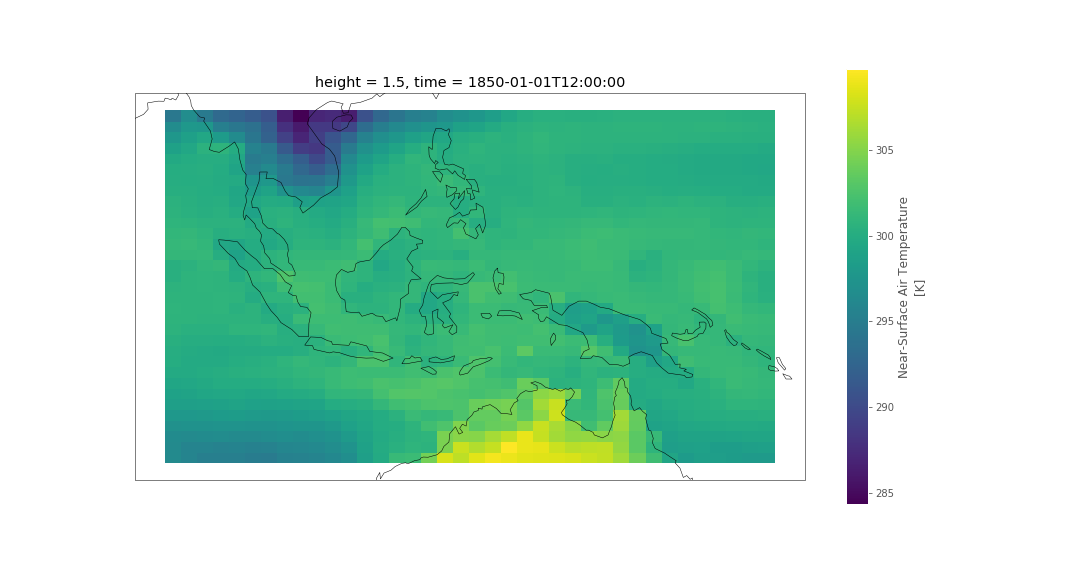
\includegraphics[width=1\textwidth]{gambar20.png}
\end{figure}

\section{Menyimpan data dalam format NetCDF}
Mengawali pembahasan ini, kita akan membuka kembali data temperatur udara dekat permukaan yang berformat NetCDF dan menyimpannya dalam bentuk dataset, untuk kemudian diekstraksi menjadi \verb|DataArray|:
\begin{lstlisting}[language=Python]
import xarray as xr
ds = xr.open_dataset('tas_Amon_ACCESS1-3_historical_r1i1p1_185001-200512.nc')
tas = ds['tas']
\end{lstlisting}

Misalkan kita hendak mengekstraksi data klimatologi temperatur udara dekat permukaan global (Januari 1961 - Desember 1990) menjadi data berformat NetCDF, maka kita dapat melakukannya dengan perintah sebagai berikut:

\begin{lstlisting}[language=Python]
tas_klim = tas.sel(time=slice('1961-01','1990-12')).mean(dim='time')
tas_klim.to_dataset(name='tas_klimatologi').to_netcdf('tas_klim.nc')
\end{lstlisting}

Untuk kembali membukanya, kita jalankan perintah sebagai berikut:

\begin{lstlisting}[language=Python]
tas_klim = xr.open_dataset('tas_klim.nc')
print(tas_klim)
\end{lstlisting}
Berikut adalah tampilan metadata-nya:
\begin{lstlisting}[numbers=none]
<xarray.Dataset>
Dimensions:          (lat: 145, lon: 192)
Coordinates:
  * lat              (lat) float64 -90.0 -88.75 -87.5 -86.25 ... 87.5 88.75 90.0
  * lon              (lon) float64 0.0 1.875 3.75 5.625 ... 354.4 356.2 358.1
    height           float64 ...
Data variables:
    tas_klimatologi  (lat, lon) float32 ...
\end{lstlisting}

\verb|xarray| menyimpan sebagian metadata dari file ke dalam objek \textit{dictionary} yang dikenal sebagai \verb|encoding|, ketika membuka data NetCDF. Objek ini juga akan diwariskan ke data NetCDF yang diekstraksi dari dataset sebelumnya. Seperti pada contoh berikut ini:

\begin{lstlisting}[language=Python]
print(ds.encoding)
\end{lstlisting}

\begin{lstlisting}[numbers=none]
{'unlimited_dims': {'time'}, 'source': '/home/ronggolawe/coding_repo/tes/tas_Amon_ACCESS1-3_historical_r1i1p1_185001-200512.nc'}
\end{lstlisting}

\begin{lstlisting}[language=Python]
print(tas.encoding)
\end{lstlisting}

\begin{lstlisting}[numbers=none]
{'source': '/home/ronggolawe/coding_repo/tes/tas_Amon_ACCESS1-3_historical_r1i1p1_185001-200512.nc', 'original_shape': (1872, 145, 192), 'dtype': dtype('float32'), 'missing_value': 1e+20, '_FillValue': 1e+20, 'coordinates': 'height'}
\end{lstlisting}
Setiap variabel dan koordinat di dalam suatu dataset mempunyai atribut \verb|encoding| - nya masing - masing. Salah satu \verb|encoding| yang menarik dapat kita jumpai pada koordinat waktu. \verb|encoding| ini berfungsi untuk mengubah objek \textit{array} numerik pada data NetCDF menjadi objek \verb|datetime| ketika kita memerintahkan pembacaan data NetCDF melalui \verb|xarray|, dan melakukan hal sebaliknya ketika kita hendak menuliskan dataset ke dalam bentuk NetCDF. Berikut adalah objek \verb|encoding| koordinat waktu pada variabel \verb|ds|:
\begin{lstlisting}[language=Python]
print(ds.time.encoding)
\end{lstlisting}

\begin{lstlisting}[numbers=none]
{'source': '/home/ronggolawe/coding_repo/tes/tas_Amon_ACCESS1-3_historical_r1i1p1_185001-200512.nc', 'original_shape': (1872,), 'dtype': dtype('float64'), 'units': 'days since 0001-01-01', 'calendar': 'proleptic_gregorian'}
\end{lstlisting}

\chapter{Studi Kasus}
\section{Visualisasi tren spasial curah hujan di Benua Maritim}
Pada bagian ini kita akan mencoba menerapkan seluruh konsep yang telah kita pelajari sebelumnya untuk menampilkan rata -rata anomali curah hujan bulanan historis dari luaran model iklim ACCESS-1.3 selama 16 tahun terakhir dari periode data (Januari 1990 - Desember 2005).

Untuk mengawali pembahasan ini, kita wajib untuk mengimpor beberapa pustaka di lingkungan komputasi ilmiah Python:
\begin{lstlisting}[language=Python]
import xarray as xr
import matplotlib.pyplot as plt
import cartopy.crs as ccrs
plt.style.use('ggplot')
%matplotlib inline
\end{lstlisting}
Kemudian, kita buka file NetCDF-nya:
\begin{lstlisting}[language=Python]
ds = xr.open_dataset('pr_Amon_ACCESS1-3_historical_r1i1p1_185001-200512.nc')
print(ds)
\end{lstlisting}
Berikut ini merupakan tampilan metadata dari dataset curah hujan tersebut:
\begin{lstlisting}[numbers=none]
<xarray.Dataset>
Dimensions:    (bnds: 2, lat: 145, lon: 192, time: 1872)
Coordinates:
  * time       (time) datetime64[ns] 1850-01-16T12:00:00 ... 2005-12-16T12:00:00
  * lat        (lat) float64 -90.0 -88.75 -87.5 -86.25 ... 86.25 87.5 88.75 90.0
  * lon        (lon) float64 0.0 1.875 3.75 5.625 ... 352.5 354.4 356.2 358.1
Dimensions without coordinates: bnds
Data variables:
    time_bnds  (time, bnds) datetime64[ns] ...
    lat_bnds   (lat, bnds) float64 ...
    lon_bnds   (lon, bnds) float64 ...
    pr         (time, lat, lon) float32 ...
Attributes:
    institution:            CSIRO (Commonwealth Scientific and Industrial Res...
    institute_id:           CSIRO-BOM
    experiment_id:          historical
    source:                 ACCESS1-3 2011. Atmosphere: AGCM v1.0 (N96 grid-p...
    model_id:               ACCESS1.3
    forcing:                GHG, Oz, SA, Sl, Vl, BC, OC, (GHG = CO2, N2O, CH4...
    parent_experiment_id:   piControl
    parent_experiment_rip:  r1i1p1
    branch_time:            90945.0
    contact:                The ACCESS wiki: http://wiki.csiro.au/confluence/...
    history:                CMIP5 compliant file produced from raw ACCESS mod...
    references:             See http://wiki.csiro.au/confluence/display/ACCES...
    initialization_method:  1
    physics_version:        1
    tracking_id:            26bfc8da-78ff-4b10-9e13-24492c09bb59
    version_number:         v20120413
    product:                output
    experiment:             historical
    frequency:              mon
    creation_date:          2012-02-08T06:45:54Z
    Conventions:            CF-1.4
    project_id:             CMIP5
    table_id:               Table Amon (27 April 2011) 9c851218e3842df9a62ef3...
    title:                  ACCESS1-3 model output prepared for CMIP5 historical
    parent_experiment:      pre-industrial control
    modeling_realm:         atmos
    realization:            1
    cmor_version:           2.8.0
\end{lstlisting}
Kemudian kita wajib mengekstraksikan \verb|DataArray| curah hujan dari dataset tersebut:
\begin{lstlisting}[language=Python]
pr = ds['pr']
print(pr)
\end{lstlisting}
Berikut ini merupakan tampilan metadata dari \verb|DataArray| curah hujan yang baru saja kita ekstraksi:
\begin{lstlisting}[numbers=none]
<xarray.DataArray 'pr' (time: 1872, lat: 145, lon: 192)>
[52116480 values with dtype=float32]
Coordinates:
  * time     (time) datetime64[ns] 1850-01-16T12:00:00 ... 2005-12-16T12:00:00
  * lat      (lat) float64 -90.0 -88.75 -87.5 -86.25 ... 86.25 87.5 88.75 90.0
  * lon      (lon) float64 0.0 1.875 3.75 5.625 7.5 ... 352.5 354.4 356.2 358.1
Attributes:
    standard_name:     precipitation_flux
    long_name:         Precipitation
    comment:           at surface; includes both liquid and solid phases from...
    units:             kg m-2 s-1
    cell_methods:      time: mean
    cell_measures:     area: areacella
    history:           2012-02-08T06:45:54Z altered by CMOR: replaced missing...
    associated_files:  baseURL: http://cmip-pcmdi.llnl.gov/CMIP5/dataLocation...
\end{lstlisting}
Karena satuan \verb|DataArray| curah hujannya masih dalam $kg.m^{-2}.s^{-1}$ ($mm.s^{-1}$), kita perlu mengubahnya menjadi $mm.bulan^{-1}$:
\begin{lstlisting}[language=Python]
pr = pr*30*24*3600
print(pr)
\end{lstlisting}
Hasilnya adalah sebagai berikut:
\begin{lstlisting}[numbers=none]
<xarray.DataArray 'pr' (time: 1872, lat: 145, lon: 192)>
array([[[ 9972244.47294138,  9972244.47294138,  9972244.47294138, ...,
          9968538.51084597,  9968538.51084597,  9968538.51084597],
        [12997152.77901851, 12904844.38184649, 12712583.46782997, ...,
         12559140.44450037, 12749926.4589278 , 12755151.62106603],
        [16683529.49107066, 16999856.11718148, 17511141.40218124, ...,
         15274677.29570344, 15777598.96055795, 16223015.58125764],
        ...,
        [47712761.87337935, 47352947.47771695, 47888491.08014256, ...,
         47106630.84452972, 47228224.89682585, 47222251.97358057],
        [40539849.32368621, 40602597.09740058, 40450930.67502603, ...,
         39993041.18519649, 40274327.6800029 , 40362601.68068111],
        [35372467.19794348, 35372467.19794348, 35372467.19794348, ...,
         35372467.19794348, 35372467.19794348, 35372467.19794348]],

       [[15765477.43985429, 15765477.43985429, 15765477.43985429, ...,
         15764178.97827923, 15764178.97827923, 15764178.97827923],
        [12538239.03214652, 12313008.65113735, 12117958.33613724, ...,
         13278118.47743578, 12984796.00762948, 12752275.91057774],
        [10178303.45069524,  9738562.63468042,  9338995.45599706, ...,
         11568405.09711765, 11098266.53182972, 10607232.66459536],
        ...,
        [37618188.57165053, 35968995.72154507, 34429826.86730102, ...,
         41677072.52316177, 40503504.62039933, 39264152.07143873],
        [32863714.17157352, 32467008.19116086, 32047094.88339722, ...,
         32890303.60942706, 32749144.03259754, 32728909.41845253],
        [16911111.61513254, 16911111.61513254, 16911111.61513254, ...,
         16911111.61513254, 16911111.61513254, 16911111.61513254]],

       [[11669375.76059718, 11669375.76059718, 11669375.76059718, ...,
         11668389.69360106, 11668389.69360106, 11668389.69360106],
        [16203712.80424297, 16155877.47981772, 16145718.92749518, ...,
         16419436.15511991, 16354390.86821862, 16308976.79273039],
        [21202889.16234858, 21002961.2146318 , 20679848.98108989, ...,
         21546439.18108195, 21453296.71329819, 21281073.35278764],
        ...,
        [22259978.95142063, 22482516.93416387, 22607720.70963867, ...,
         22625659.3381986 , 22535876.06688961, 22499048.64141718],
        [19393954.98647355, 19038763.11401837, 18903729.22061943, ...,
         20362237.64182068, 20058681.76720105, 19714247.26699479],
        [21202085.6437739 , 21202085.6437739 , 21202085.6437739 , ...,
         21202085.6437739 , 21202085.6437739 , 21202085.6437739 ]],

       ...,

       [[10385059.01489407, 10385059.01489407, 10385059.01489407, ...,
         10385854.89545949, 10385854.89545949, 10385854.89545949],
        [13380168.39162447, 13325674.25072193, 13252143.13552715, ...,
         13486518.50502938, 13439081.88468777, 13402957.15606771],
        [16489177.29011737, 16355784.04110856, 16149933.58100764, ...,
         16554880.97341731, 16620552.57707834, 16598468.03708933],
        ...,
        [52850789.60191458, 55634648.44599366, 57659979.64516282, ...,
         47354129.84155118, 49111522.73090556, 50760113.70588094],
        [64274116.82344973, 64619214.3028602 , 65401065.37286192, ...,
         63084554.92928624, 63275492.94009805, 63243651.60707384],
        [62822290.13275355, 62822290.13275355, 62822290.13275355, ...,
         62822290.13275355, 62822290.13275355, 62822290.13275355]],

       [[17331185.32109074, 17331185.32109074, 17331185.32109074, ...,
         17320701.38957351, 17320701.38957351, 17320701.38957351],
        [15471524.0704827 , 15346457.77917467, 15627586.93099022, ...,
         15943268.90911907, 15743243.19488369, 15679369.57860366],
        [16980313.50667588, 16860016.38835296, 16813971.41329944, ...,
         17523452.34551467, 17030658.68094563, 17039874.70292486],
        ...,
        [91745011.49822026, 91251528.88521552, 90534136.50300354, ...,
         94346969.62404996, 94393867.00093746, 92597456.10505342],
        [86219088.99676055, 85681758.10016692, 84742973.43660146, ...,
         88392835.88156104, 87694954.03021574, 87045436.05353683],
        [69958647.17010409, 69958647.17010409, 69958647.17010409, ...,
         69958647.17010409, 69958647.17010409, 69958647.17010409]],

       [[ 9347095.56482267,  9347095.56482267,  9347095.56482267, ...,
          9344911.09417286,  9344911.09417286,  9344911.09417286],
        [ 6043097.83730423,  6054329.91182897,  6069176.67423841, ...,
          6074991.87259236,  6038992.02542379,  6004887.16835389],
        [ 6163002.74385139,  6092734.96811511,  5988925.25659176, ...,
          6265302.42094304,  6229572.577402  ,  6229823.10410589],
        ...,
        [66317394.28918809, 64711890.8520788 , 63606139.30597901, ...,
         65125314.90717083, 66816351.82723403, 67544852.93012112],
        [49903312.37856299, 50660034.39808264, 51353855.88370264, ...,
         48003565.32773003, 48843947.9903318 , 49570756.51036575],
        [44999435.46205759, 44999435.46205759, 44999435.46205759, ...,
         44999435.46205759, 44999435.46205759, 44999435.46205759]]])
Coordinates:
  * time     (time) datetime64[ns] 1850-01-16T12:00:00 ... 2005-12-16T12:00:00
  * lat      (lat) float64 -90.0 -88.75 -87.5 -86.25 ... 86.25 87.5 88.75 90.0
  * lon      (lon) float64 0.0 1.875 3.75 5.625 7.5 ... 352.5 354.4 356.2 358.1
\end{lstlisting}

Selanjutnya, kita mengekstraksi \verb|DataArray| pada koordinat Benua Maritim:
\begin{lstlisting}[language=Python]
pr_bm = pr.sel(lat=slice(-20,20),lon=slice(90,160))
print(pr_bm)
\end{lstlisting}
Hasilnya:
\begin{lstlisting}[numbers=none]
<xarray.DataArray 'pr' (time: 1872, lat: 33, lon: 38)>
array([[[3.27974161e+01, 2.69479198e+01, 2.16606988e+01, ...,
         5.30489683e+01, 5.80844767e+01, 5.05003862e+01],
        [3.24819498e+01, 2.55849736e+01, 1.82543624e+01, ...,
         9.48242726e+01, 6.59841397e+01, 5.27378137e+01],
        [2.01826262e+01, 1.87158432e+01, 1.94405346e+01, ...,
         7.91689373e+01, 7.33096648e+01, 5.76325235e+01],
        ...,
        [1.83752139e+01, 2.84630439e+01, 3.01624444e+01, ...,
         3.92409940e+01, 3.07302714e+01, 3.00869577e+01],
        [1.69064518e+01, 1.62390949e+01, 1.06508562e+01, ...,
         7.68419423e+01, 5.44062802e+01, 4.40820067e+01],
        [1.65910020e+01, 1.61794701e+01, 1.26975999e+01, ...,
         6.68837887e+01, 6.08938969e+01, 6.21407594e+01]],

       [[3.01312794e+01, 2.43283372e+01, 1.72953161e+01, ...,
         4.98849606e+01, 5.27583514e+01, 3.98192290e+01],
        [2.43714778e+01, 2.34348151e+01, 2.56363345e+01, ...,
         4.42819151e+01, 4.97231244e+01, 5.84556227e+01],
        [2.34119270e+01, 2.33271757e+01, 2.49248893e+01, ...,
         6.36581726e+01, 8.99394262e+01, 1.09775525e+02],
        ...,
        [8.71310327e+00, 3.22348921e+00, 1.24815400e+00, ...,
         8.10774872e+01, 9.47482791e+01, 1.01101075e+02],
        [1.10434145e+01, 6.26409760e+00, 8.48107259e-02, ...,
         6.36822606e+01, 6.40597008e+01, 7.55018866e+01],
        [5.55906809e+00, 6.04082373e+00, 2.10051369e-01, ...,
         5.78729935e+01, 4.16069569e+01, 3.44678912e+01]],

       [[4.14911043e+01, 2.78626751e+01, 2.48405294e+01, ...,
         3.82862829e+01, 5.02943249e+01, 6.20464819e+01],
        [2.89406929e+01, 2.52717162e+01, 2.30385698e+01, ...,
         3.97911475e+01, 5.46255382e+01, 6.36811337e+01],
        [2.61719452e+01, 3.03813205e+01, 3.91469592e+01, ...,
         4.76275093e+01, 5.18427474e+01, 5.19740929e+01],
        ...,
        [8.15364561e+00, 9.70090532e+00, 2.58854727e+00, ...,
         8.66233609e+01, 8.19169893e+01, 9.55829626e+01],
        [9.04263976e+00, 1.07825294e+01, 3.44861717e+00, ...,
         9.25600932e+01, 7.83239330e+01, 9.46521722e+01],
        [2.39509300e+01, 1.40617743e+01, 3.25027145e+00, ...,
         1.03732983e+02, 9.85868879e+01, 9.49117702e+01]],

       ...,

       [[4.59701744e+01, 4.76911405e+01, 4.54319305e+01, ...,
         2.14848030e+01, 2.07870756e+01, 2.22414728e+01],
        [5.13943680e+01, 4.26593001e+01, 4.14484729e+01, ...,
         2.23991576e+01, 1.95551861e+01, 2.43836067e+01],
        [5.26504952e+01, 5.02504064e+01, 4.22745001e+01, ...,
         3.53254557e+01, 2.98879192e+01, 2.49001436e+01],
        ...,
        [4.24207906e+02, 3.09004265e+02, 1.65305757e+02, ...,
         1.26857876e+02, 9.84617943e+01, 8.22557963e+01],
        [3.64153615e+02, 2.44217048e+02, 1.33914897e+02, ...,
         1.63156119e+02, 1.46704045e+02, 1.11266134e+02],
        [1.84446797e+02, 1.16533126e+02, 9.61965588e+01, ...,
         1.57720214e+02, 8.29196996e+01, 9.93205329e+01]],

       [[4.21528860e+01, 3.92910606e+01, 3.88421602e+01, ...,
         3.13487380e+01, 2.98476971e+01, 2.43801272e+01],
        [4.26347265e+01, 4.30019073e+01, 4.24465344e+01, ...,
         3.16284047e+01, 3.35953241e+01, 3.27928875e+01],
        [4.13478445e+01, 3.53408567e+01, 3.43819706e+01, ...,
         3.46018416e+01, 3.45193699e+01, 3.44043590e+01],
        ...,
        [9.73465412e+01, 1.70275272e+02, 1.33757554e+02, ...,
         2.67322191e+01, 2.35591449e+01, 2.58952866e+01],
        [1.23357499e+02, 2.35845903e+02, 1.47469082e+02, ...,
         7.42893715e+01, 6.77664597e+01, 6.41992925e+01],
        [8.13584622e+01, 1.26756413e+02, 1.41154391e+02, ...,
         9.30234846e+01, 7.26195848e+01, 6.44770426e+01]],

       [[4.05248490e+01, 3.47790245e+01, 3.06977227e+01, ...,
         4.44322188e+01, 3.76007362e+01, 2.46168866e+01],
        [4.14995062e+01, 3.65583742e+01, 4.06294096e+01, ...,
         2.70747343e+01, 2.99497565e+01, 3.19751349e+01],
        [3.90298949e+01, 4.07663846e+01, 2.82636140e+01, ...,
         3.37559604e+01, 3.76480518e+01, 3.54408109e+01],
        ...,
        [8.72914250e+00, 4.73530613e+00, 1.33957614e+00, ...,
         4.89995692e+01, 5.44041963e+01, 5.44323437e+01],
        [5.74322780e+00, 3.38408749e+00, 2.61762534e+00, ...,
         4.57096099e+01, 5.21575984e+01, 5.55414676e+01],
        [8.41005052e+00, 1.61640712e+00, 1.00369438e+00, ...,
         5.76550509e+01, 4.64409163e+01, 4.70227817e+01]]])
Coordinates:
  * time     (time) datetime64[ns] 1850-01-16T12:00:00 ... 2005-12-16T12:00:00
  * lat      (lat) float64 -20.0 -18.75 -17.5 -16.25 ... 16.25 17.5 18.75 20.0
  * lon      (lon) float64 90.0 91.88 93.75 95.62 ... 153.8 155.6 157.5 159.4
\end{lstlisting}

Data curah hujan sepanjang Januari 1961 - Desember 1990 kita jadikan patokan untuk mengukur anomali curah hujan modern di Benua Maritim:
\begin{lstlisting}[language=Python]
pr_bm_klim = pr_bm.sel(time=slice('1961-01','1990-12')).mean(dim='time')
pr_bm_anom = pr_bm - pr_bm_klim
\end{lstlisting}
Untuk kemudian kita ekstraksi hanya pada periode Januari 1990 - Desember 2005:
\begin{lstlisting}[language=Python]
pr_bm_anom_mod = pr_bm_anom.sel(time=slice('1990-01', None))
\end{lstlisting}
Selanjutnya, dengan menggunakan metode \verb|groupby()|, kita kelompokan berdasarkan rata - rata anomali curah hujan bulanannya dan kita tampilkan dalam bentuk visual:
\begin{lstlisting}[language=Python]
plt.figure(figsize=(40,30));
proj = ccrs.PlateCarree();
pr_anom_bul = pr_bm_anom_mod.groupby('time.month').mean(dim='time')
p = pr_anom_bul.plot(col='month',col_wrap=6,
                subplot_kws=dict(projection=proj),
                transform=ccrs.PlateCarree(),
                cmap = 'bwr_r);

for ax in p.axes.flat:
    ax.coastlines();
\end{lstlisting}

\begin{figure}[H]
    \centering
    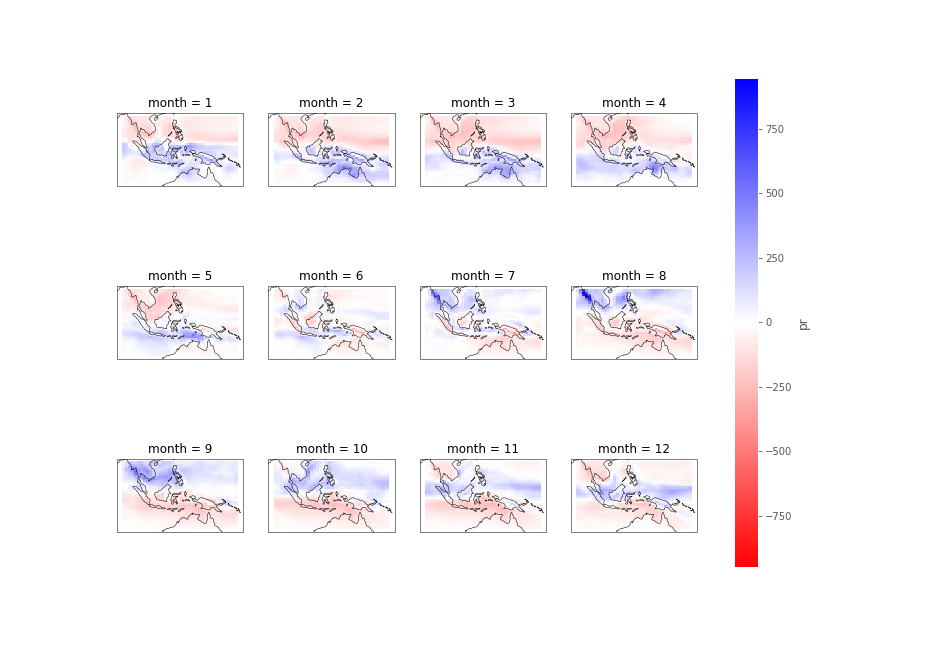
\includegraphics[width=1.5\textwidth]{gambar21.png}
\end{figure}

\section{Perhitungan indeks Ni{\~{n}}o 3.4}
Pada bagian ini kita akan mencoba melakukan perhitungan indeks Ni{\~{n}}o 3.4, yang mana merupakan salah satu indikator El Ni{\~{n}}o yang cukup populer di kalangan geosaintis, dengan menggunakan data historis temperatur permukaan laut yang kita peroleh dari model yang telah kita bahas pada bagian - bagian sebelumnya.

Indeks Ni{\~{n}}o 3.4 dapat didefinisikan sebagai anomali rata - rata temperatur permukaan laut di Pasifik ekuator mulai dari wilayah batas penanggalan internasional, hingga lepas pantai Amerika Selatan (5$^{\circ}$ LU - 5$^{\circ}$ LS, 170$^{\circ}$ BB - 120 $^{\circ}$ BB)\footnote{\url{https://www.cpc.ncep.noaa.gov/products/analysis_monitoring/ensostuff/nino_regions.shtml}}. Indeks Ni{\~{n}}o 3.4 umumnya didefinisikan sebagai rata - rata bergerak lima bulanan (\textit{5-month running mean}) dan fenomena El Ni{\~{n}}o dan La Ni{\~{n}}a didefinisikan ketika terjadi perubahan sebesar $\pm 0,4^{\circ}$C untuk periode enam bulan atau lebih\footnote{\url{https://climatedataguide.ucar.edu/climate-data/nino-sst-indices-nino-12-3-34-4-oni-and-tni}}.

Berikut merupakan langkah - langkah yang akan kita lakukan untuk menghitung indeks Ni{\~{n}}o 3.4:
\begin{enumerate}
    \item Menghitung rata - rata spasial dari temperatur permukaan laut di wilayah Ni{\~{n}}o 3.4 sepanjang periode data.\label{1}
    \item Menghitung rata - rata spasial klimatologi (30 tahunan) dari temperatur permukaan laut di wilayah Ni{\~{n}}o 3.4.\label{2}
    \item Menghitung anomali rata - rata spasial temperatur permukaan laut dengan mengurangi data dari hasil perhitungan \ref{1} ke data yang dijadikan acuan klimatologi pada perhitungan \ref{2}. \label{3}
    \item Menghaluskan (\textit{smoothing}) hasil perhitungan no. \ref{3} dengan menggunakan rata - rata bergerak lima bulanan. \label{4}
    \item Menormalisasi hasil perhitungan no. \ref{4} terhadap standar deviasi sepanjang periode iklim yang dijadikan acuan.
\end{enumerate}

Langkah awal yang hendak kita lakukan adalah mengimpor beberapa pustaka yang digunakan di dalam perhitungan:
\begin{lstlisting}[language=Python]
import xarray as xr
import matplotlib.pyplot as plt
import cartopy.crs as ccrs
plt.style.use('ggplot')
%matplotlib inline
\end{lstlisting}
Kita kemudian membuka dataset temperatur permukaan laut global bulanan dari file NetCDF:
\begin{lstlisting}[language=Python]
ds = xr.open_dataset('tos_Omon_ACCESS1-3_historical_r1i1p1_185001-200512.nc')
print(ds)
\end{lstlisting}
dan memeriksa metadata di dalamnya:
\begin{lstlisting}[numbers=none]
<xarray.Dataset>
Dimensions:       (bnds: 2, i: 360, j: 300, time: 1872, vertices: 4)
Coordinates:
  * time          (time) datetime64[ns] 1850-01-16T12:00:00 ... 2005-12-16T12:00:00
  * j             (j) int32 0 1 2 3 4 5 6 7 ... 292 293 294 295 296 297 298 299
  * i             (i) int32 0 1 2 3 4 5 6 7 ... 352 353 354 355 356 357 358 359
    lat           (j, i) float32 ...
    lon           (j, i) float32 ...
Dimensions without coordinates: bnds, vertices
Data variables:
    time_bnds     (time, bnds) datetime64[ns] ...
    lat_vertices  (j, i, vertices) float32 ...
    lon_vertices  (j, i, vertices) float32 ...
    tos           (time, j, i) float32 ...
Attributes:
    institution:            CSIRO (Commonwealth Scientific and Industrial Res...
    institute_id:           CSIRO-BOM
    experiment_id:          historical
    source:                 ACCESS1-3 2011. Atmosphere: AGCM v1.0 (N96 grid-p...
    model_id:               ACCESS1.3
    forcing:                GHG, Oz, SA, Sl, Vl, BC, OC, (GHG = CO2, N2O, CH4...
    parent_experiment_id:   piControl
    parent_experiment_rip:  r1i1p1
    branch_time:            90945.0
    contact:                The ACCESS wiki: http://wiki.csiro.au/confluence/...
    history:                CMIP5 compliant file produced from raw ACCESS mod...
    references:             See http://wiki.csiro.au/confluence/display/ACCES...
    initialization_method:  1
    physics_version:        1
    tracking_id:            133724da-4e35-4a17-811a-36891ab0d95d
    version_number:         v20120413
    product:                output
    experiment:             historical
    frequency:              mon
    creation_date:          2012-02-06T01:20:17Z
    Conventions:            CF-1.4
    project_id:             CMIP5
    table_id:               Table Omon (27 April 2011) 694b38a3f68f18e58ba802...
    title:                  ACCESS1-3 model output prepared for CMIP5 historical
    parent_experiment:      pre-industrial control
    modeling_realm:         ocean
    realization:            1
    cmor_version:           2.8.0
\end{lstlisting}

Kemudian kita melakukan ekstraksi data \verb|tos| global untuk periode Januari 1961 hingga akhir periode data:
\begin{lstlisting}[language=Python]
tos = ds['tos'].sel(time=slice('1961-01', None))
print(tos)
\end{lstlisting}
Berikut adalah tampilan metadata-nya:
\begin{lstlisting}
<xarray.DataArray 'tos' (time: 540, j: 300, i: 360)>
[58320000 values with dtype=float32]
Coordinates:
  * time     (time) datetime64[ns] 1961-01-16T12:00:00 ... 2005-12-16T12:00:00
  * j        (j) int32 0 1 2 3 4 5 6 7 8 ... 291 292 293 294 295 296 297 298 299
  * i        (i) int32 0 1 2 3 4 5 6 7 8 ... 351 352 353 354 355 356 357 358 359
    lat      (j, i) float32 ...
    lon      (j, i) float32 ...
Attributes:
    standard_name:     sea_surface_temperature
    long_name:         Sea Surface Temperature
    comment:           "this may differ from ""surface temperature"" in regio...
    units:             K
    cell_methods:      time: mean
    cell_measures:     area: areacello
    history:           2012-02-06T01:20:16Z altered by CMOR: replaced missing...
    associated_files:  baseURL: http://cmip-pcmdi.llnl.gov/CMIP5/dataLocation...
\end{lstlisting}
Karena temperatur permukaan laut masih dalam satuan Kelvin, kita dapat mengubahnya menjadi $^{\circ}$C:
\begin{lstlisting}[language=Python]
tas = tas - 273.15
\end{lstlisting}
Untuk memeriksa validitas data secara kualitatif, ada baiknya kita memvisualisasikan data pada \textit{timestamp} pertama:
\begin{lstlisting}[language=Python]
plot1 = tos.isel(time=0).plot(size=8);
\end{lstlisting}
\begin{figure}[H]
    \centering
    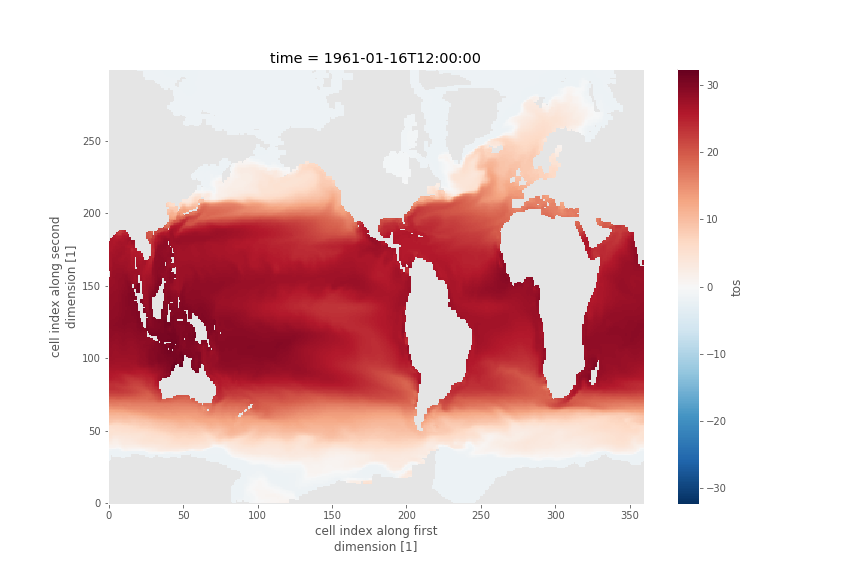
\includegraphics[width=1\textwidth]{gambar22.png}
\end{figure}

Komponen oseanik di dalam model ACCESS 1-3 dibangun di atas MOM5\footnote{Collier M, Uhe P (2012) CMIP5 datasets from the ACCESS1.0 and ACCESS1.3 coupled climate models. CAWCR Technical Report No. 059. The Centre for Australian Weather and Climate Research. \url{https://cawcr.gov.au/technical-reports/CTR_059.pdf}}. MOM5 sendiri mempunyai sistem \textit{tripolar grid}(seperti pada gambar di halaman selanjutnya)\footnote{Griffies, S., 2012: Elements of the Modular Ocean Model (MOM). NOAA GFDL Ocean Group Tech. Rep. 7, 618 pp.\url{http://www.mom-ocean.org/web/docs/project/MOM5_elements.pdf}}. Dengan demikian, berarti terdapat tiga buah kutub (satu kutub di selatan dan dua buah kutub di utara) yang digunakan dalam konfigurasi koordinat model ini. Dengan demikian, terdapat dua komponen sistem koordinat tambahan di luar \verb|lat| dan \verb|lon|, yakni \verb|i| dan \verb|j| di dalam konfigurasi model ini. Sistem koordinat tambahan itu baru berpengaruh jika kita hendak mengekstraksi data di atas lintang 60$^{\circ}$, yang mana dalam kasus ini kita tidak begitu terpengaruh, namun dengan adanya koordinat \textit{tripolar grid} ini, kita harus mengekstraksi \verb|DataArray| dengan cara yang sedikit berbeda.
\begin{figure}[H]
    \centering
    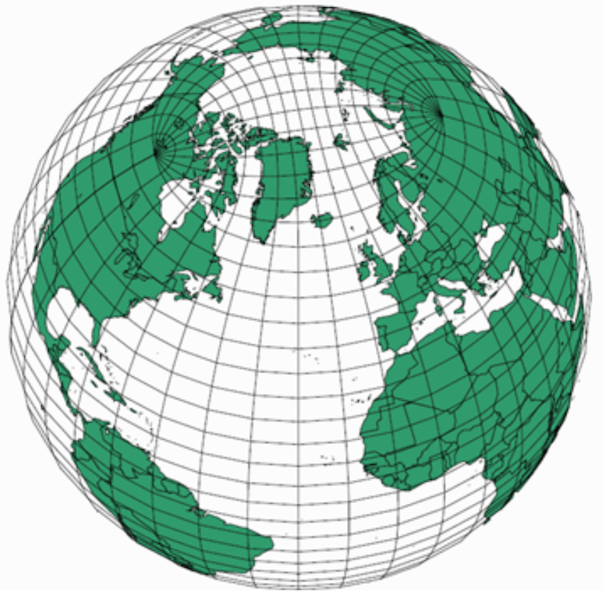
\includegraphics[width=.8\textwidth]{gambar23.png}
\end{figure}
Terdapat tiga cara yang dapat kita lakukan untuk mengekstraksi \verb|DataArray| pada wilayah yang kita kehendaki:
\begin{enumerate}
    \item Ekstraksi dengan menggunakan metode \verb|sel()| untuk seluruh komponen di dalam koordinat \textit{tripolar grid}.
    \item Membuang koordinat \verb|i| dan \verb|j| dan mendefinisikan sistem koordinat ulang.
    \item Menggunakan operator logika di dalam metode \verb|where()| untuk menyeleksi wilayah yang kita kehendaki.
\end{enumerate}
Dari ketiga cara tersebut, cara no. 3 merupakan cara yang paling mudah. Oleh karena itu kita akan menggunakan cara ini:
\begin{lstlisting}[language=Python]
tos_nino34 = tos.where((tos['lat'] < 5) & (tos['lat'] > -5) & (tos['lon'] > 190) & (tos['lon'] < 240),drop=True)
print(tos_nino34)
\end{lstlisting}

\begin{lstlisting}[numbers=none]
<xarray.DataArray 'tos' (time: 540, j: 30, i: 50)>
array([[[28.205902, 28.077667, 27.951202, ..., 24.75177 , 24.604523,
         24.379639],
        [27.9234  , 27.809052, 27.714508, ..., 24.43805 , 24.30252 ,
         24.150177],
        [27.67038 , 27.586761, 27.519623, ..., 24.212036, 24.117676,
         24.029785],
        ...,
        [27.347443, 27.319305, 27.243011, ..., 26.490051, 26.680817,
         26.876953],
        [27.411865, 27.381226, 27.314392, ..., 27.118835, 27.048767,
         27.073029],
        [27.51065 , 27.473969, 27.43573 , ..., 27.686188, 27.612732,
         27.519012]],

       [[27.671814, 27.688416, 27.74231 , ..., 25.570496, 25.589874,
         25.619598],
        [27.52945 , 27.578827, 27.641266, ..., 25.59787 , 25.637878,
         25.671722],
        [27.410645, 27.463379, 27.519714, ..., 25.645813, 25.690826,
         25.723236],
        ...,
        [26.956543, 26.786163, 26.581757, ..., 27.481384, 27.492828,
         27.445496],
        [27.123901, 27.010681, 26.823761, ..., 27.6008  , 27.61148 ,
         27.572113],
        [27.245148, 27.203278, 27.088898, ..., 27.661835, 27.675293,
         27.647522]],

       [[27.445587, 27.109985, 26.818237, ..., 26.897858, 26.876404,
         26.858765],
        [27.096619, 26.74881 , 26.471527, ..., 26.960663, 26.944153,
         26.930328],
        [26.825592, 26.529816, 26.340668, ..., 27.009613, 26.998718,
         26.989563],
        ...,
        [27.122559, 27.156342, 27.144073, ..., 27.460388, 27.368408,
         27.256561],
        [27.186646, 27.235046, 27.24759 , ..., 27.468933, 27.383331,
         27.281647],
        [27.28122 , 27.308228, 27.325012, ..., 27.472656, 27.390625,
         27.299347]],

       ...,

       [[29.720764, 29.717865, 29.71579 , ..., 25.338654, 25.194519,
         25.066559],
        [29.583344, 29.582214, 29.57196 , ..., 25.222412, 25.098694,
         24.978455],
        [29.426453, 29.421875, 29.404205, ..., 25.137573, 25.009705,
         24.891693],
        ...,
        [29.245605, 29.22821 , 29.236267, ..., 28.039062, 27.8508  ,
         27.679413],
        [29.559937, 29.519623, 29.509827, ..., 28.381256, 28.241943,
         28.102142],
        [29.867462, 29.82721 , 29.803192, ..., 28.645355, 28.557281,
         28.457214]],

       [[29.643158, 29.662842, 29.672394, ..., 25.450317, 25.397095,
         25.281067],
        [29.526093, 29.525574, 29.481262, ..., 25.25055 , 25.215363,
         25.117035],
        [29.362488, 29.3031  , 29.19632 , ..., 25.073395, 25.057251,
         24.972595],
        ...,
        [29.277496, 29.254974, 29.219849, ..., 28.198975, 28.135284,
         28.1492  ],
        [29.488312, 29.460846, 29.427032, ..., 28.522186, 28.477234,
         28.487823],
        [29.67221 , 29.658936, 29.640228, ..., 28.747833, 28.7247  ,
         28.733246]],

       [[29.43628 , 29.400604, 29.324066, ..., 25.582611, 25.461945,
         25.3667  ],
        [29.188446, 29.11142 , 29.024078, ..., 25.397247, 25.288483,
         25.210907],
        [28.913757, 28.819336, 28.725677, ..., 25.251007, 25.163116,
         25.101929],
        ...,
        [28.63678 , 28.599548, 28.54776 , ..., 28.473145, 28.459747,
         28.354675],
        [28.836548, 28.832336, 28.823853, ..., 28.73877 , 28.749268,
         28.692078],
        [28.956085, 28.962463, 28.978882, ..., 28.893646, 28.90738 ,
         28.882751]]], dtype=float32)
Coordinates:
  * time     (time) datetime64[ns] 1961-01-16T12:00:00 ... 2005-12-16T12:00:00
  * j        (j) int32 122 123 124 125 126 127 128 ... 146 147 148 149 150 151
  * i        (i) int32 110 111 112 113 114 115 116 ... 154 155 156 157 158 159
    lat      (j, i) float32 -4.8328757 -4.8328757 ... 4.8328757 4.8328757
    lon      (j, i) float32 190.5 191.5 192.5 193.5 ... 236.5 237.5 238.5 239.5
\end{lstlisting}
Kemudian kita harus menentukan periode yang dijadikan \textit{baseline} untuk analisis klimatologi (dalam kasus ini Januari 1961 - Desember 1990). Sesudah itu, kita cari nilai rata - rata bulanannya:
\begin{lstlisting}[language=Python]
baseline = tos_nino34.sel(time=slice('1961', '1990'))
rata2baseline = baseline.groupby('time.month').mean(dim='time')
print(rata2baseline)
\end{lstlisting}
\begin{lstlisting}[numbers=none]
<xarray.DataArray 'tos' (month: 12, j: 30, i: 50)>
array([[[28.734009, 28.683922, 28.62647 , ..., 25.633846, 25.560766,
         25.505913],
        [28.576729, 28.524076, 28.46182 , ..., 25.484318, 25.437967,
         25.407549],
        [28.425814, 28.37262 , 28.308289, ..., 25.385897, 25.361462,
         25.346092],
        ...,
        [27.48979 , 27.473026, 27.45908 , ..., 28.11144 , 28.147196,
         28.171959],
        [27.553219, 27.53573 , 27.525557, ..., 28.252934, 28.28584 ,
         28.314861],
        [27.665508, 27.641302, 27.62802 , ..., 28.303043, 28.337564,
         28.367184]],

       [[28.49192 , 28.448612, 28.40968 , ..., 26.495714, 26.490767,
         26.487186],
        [28.267859, 28.223877, 28.175428, ..., 26.463076, 26.469034,
         26.475443],
        [28.053047, 28.006193, 27.952213, ..., 26.435997, 26.451412,
         26.463696],
        ...,
        [27.270794, 27.236818, 27.2098  , ..., 28.014517, 28.044697,
         28.03987 ],
        [27.30439 , 27.274403, 27.243286, ..., 28.042082, 28.074564,
         28.078747],
        [27.353737, 27.327518, 27.299482, ..., 28.041264, 28.070065,
         28.081427]],

       [[28.35741 , 28.313318, 28.285612, ..., 27.56149 , 27.557959,
         27.557096],
        [28.079899, 28.035074, 27.998657, ..., 27.505672, 27.512825,
         27.522272],
        [27.823366, 27.77669 , 27.734003, ..., 27.42212 , 27.435675,
         27.450008],
        ...,
        [27.260975, 27.248318, 27.247316, ..., 27.572004, 27.468994,
         27.356806],
        [27.280397, 27.254683, 27.246477, ..., 27.693424, 27.600391,
         27.48981 ],
        [27.320148, 27.289473, 27.27437 , ..., 27.797075, 27.719921,
         27.618322]],

       ...,

       [[29.158228, 29.124153, 29.091772, ..., 25.212542, 25.075972,
         24.925365],
        [29.044361, 29.00575 , 28.97107 , ..., 25.058813, 24.917833,
         24.771566],
        [28.910295, 28.866804, 28.827108, ..., 24.942371, 24.802662,
         24.665318],
        ...,
        [28.936438, 28.884153, 28.839474, ..., 27.425236, 27.392876,
         27.386747],
        [29.160221, 29.114998, 29.070171, ..., 27.723528, 27.680798,
         27.666609],
        [29.348507, 29.318783, 29.282091, ..., 27.964365, 27.914953,
         27.888805]],

       [[29.20702 , 29.168806, 29.137304, ..., 25.153288, 25.028482,
         24.90346 ],
        [29.095377, 29.055855, 29.01818 , ..., 24.980122, 24.863914,
         24.752176],
        [28.966837, 28.922815, 28.879068, ..., 24.84746 , 24.740788,
         24.63791 ],
        ...,
        [28.518717, 28.497175, 28.471231, ..., 27.737078, 27.745733,
         27.753435],
        [28.702515, 28.676994, 28.653309, ..., 28.031832, 28.038935,
         28.051718],
        [28.90528 , 28.881613, 28.858175, ..., 28.274109, 28.272009,
         28.278088]],

       [[29.058659, 29.012215, 28.96853 , ..., 25.34714 , 25.254887,
         25.156189],
        [28.922184, 28.872046, 28.826347, ..., 25.169653, 25.08826 ,
         25.003773],
        [28.779469, 28.732035, 28.684599, ..., 25.027555, 24.956394,
         24.880808],
        ...,
        [28.037878, 27.99222 , 27.951193, ..., 28.109655, 28.250061,
         28.340595],
        [28.161133, 28.122433, 28.084764, ..., 28.393042, 28.502478,
         28.570055],
        [28.311052, 28.277315, 28.245228, ..., 28.582253, 28.652594,
         28.697721]]], dtype=float32)
Coordinates:
  * j        (j) int32 122 123 124 125 126 127 128 ... 146 147 148 149 150 151
  * i        (i) int32 110 111 112 113 114 115 116 ... 154 155 156 157 158 159
    lat      (j, i) float32 -4.8328757 -4.8328757 ... 4.8328757 4.8328757
    lon      (j, i) float32 190.5 191.5 192.5 193.5 ... 236.5 237.5 238.5 239.5
  * month    (month) int64 1 2 3 4 5 6 7 8 9 10 11 12
\end{lstlisting}

Kemudian kita hitung anomali temperatur permukaan laut rata - rata bulanan sepanjang 1961 - 2005 dengan mengacu pada \textit{baseline} klimatologi(1961 - 1990):

\begin{lstlisting}[language=Python]
anomali = tos_nino34.groupby('time.month') - rata2baseline
print(anomali)
\end{lstlisting}

\begin{lstlisting}[numbers=none]
<xarray.DataArray 'tos' (time: 540, j: 30, i: 50)>
array([[[-5.28106689e-01, -6.06254578e-01, -6.75268173e-01, ...,
         -8.82076263e-01, -9.56243515e-01, -1.12627411e+00],
        [-6.53327942e-01, -7.15024948e-01, -7.47312546e-01, ...,
         -1.04626846e+00, -1.13544655e+00, -1.25737190e+00],
        [-7.55434036e-01, -7.85858154e-01, -7.88665771e-01, ...,
         -1.17386055e+00, -1.24378586e+00, -1.31630707e+00],
        ...,
        [-1.42347336e-01, -1.53720856e-01, -2.16068268e-01, ...,
         -1.62138939e+00, -1.46637917e+00, -1.29500580e+00],
        [-1.41353607e-01, -1.54504776e-01, -2.11164474e-01, ...,
         -1.13409805e+00, -1.23707199e+00, -1.24183273e+00],
        [-1.54857635e-01, -1.67333603e-01, -1.92289352e-01, ...,
         -6.16855621e-01, -7.24832535e-01, -8.48171234e-01]],

       [[-8.20106506e-01, -7.60196686e-01, -6.67369843e-01, ...,
         -9.25218582e-01, -9.00892258e-01, -8.67588043e-01],
        [-7.38409042e-01, -6.45050049e-01, -5.34162521e-01, ...,
         -8.65205765e-01, -8.31155777e-01, -8.03720474e-01],
        [-6.42402649e-01, -5.42814255e-01, -4.32498932e-01, ...,
         -7.90184021e-01, -7.60585785e-01, -7.40459442e-01],
        ...,
        [-3.14250946e-01, -4.50654984e-01, -6.28044128e-01, ...,
         -5.33132553e-01, -5.51868439e-01, -5.94373703e-01],
        [-1.80488586e-01, -2.63721466e-01, -4.19525146e-01, ...,
         -4.41282272e-01, -4.63083267e-01, -5.06633759e-01],
        [-1.08589172e-01, -1.24240875e-01, -2.10584641e-01, ...,
         -3.79428864e-01, -3.94771576e-01, -4.33904648e-01]],

       [[-9.11823273e-01, -1.20333290e+00, -1.46737480e+00, ...,
         -6.63631439e-01, -6.81554794e-01, -6.98331833e-01],
        [-9.83280182e-01, -1.28626442e+00, -1.52713013e+00, ...,
         -5.45009613e-01, -5.68672180e-01, -5.91943741e-01],
        [-9.97774124e-01, -1.24687386e+00, -1.39333534e+00, ...,
         -4.12506104e-01, -4.36956406e-01, -4.60445404e-01],
        ...,
        [-1.38416290e-01, -9.19761658e-02, -1.03242874e-01, ...,
         -1.11616135e-01, -1.00585938e-01, -1.00244522e-01],
        [-9.37519073e-02, -1.96361542e-02,  1.11198425e-03, ...,
         -2.24491119e-01, -2.17060089e-01, -2.08164215e-01],
        [-3.89289856e-02,  1.87549591e-02,  5.06420135e-02, ...,
         -3.24419022e-01, -3.29296112e-01, -3.18975449e-01]],

       ...,

       [[ 5.62536240e-01,  5.93711853e-01,  6.24017715e-01, ...,
          1.26111984e-01,  1.18547440e-01,  1.41193390e-01],
        [ 5.38982391e-01,  5.76463699e-01,  6.00891113e-01, ...,
          1.63599014e-01,  1.80860519e-01,  2.06888199e-01],
        [ 5.16157150e-01,  5.55070877e-01,  5.77096939e-01, ...,
          1.95201874e-01,  2.07042694e-01,  2.26375580e-01],
        ...,
        [ 3.09167862e-01,  3.44057083e-01,  3.96793365e-01, ...,
          6.13826752e-01,  4.57923889e-01,  2.92665482e-01],
        [ 3.99715424e-01,  4.04624939e-01,  4.39655304e-01, ...,
          6.57728195e-01,  5.61145782e-01,  4.35533524e-01],
        [ 5.18955231e-01,  5.08426666e-01,  5.21100998e-01, ...,
          6.80990219e-01,  6.42328262e-01,  5.68408966e-01]],

       [[ 4.36138153e-01,  4.94035721e-01,  5.35089493e-01, ...,
          2.97029495e-01,  3.68612289e-01,  3.77607346e-01],
        [ 4.30715561e-01,  4.69718933e-01,  4.63081360e-01, ...,
          2.70427704e-01,  3.51448059e-01,  3.64858627e-01],
        [ 3.95650864e-01,  3.80285263e-01,  3.17251205e-01, ...,
          2.25934982e-01,  3.16463470e-01,  3.34684372e-01],
        ...,
        [ 7.58779526e-01,  7.57799149e-01,  7.48617172e-01, ...,
          4.61896896e-01,  3.89551163e-01,  3.95765305e-01],
        [ 7.85797119e-01,  7.83851624e-01,  7.73723602e-01, ...,
          4.90354538e-01,  4.38299179e-01,  4.36105728e-01],
        [ 7.66931534e-01,  7.77322769e-01,  7.82052994e-01, ...,
          4.73724365e-01,  4.52692032e-01,  4.55158234e-01]],

       [[ 3.77620697e-01,  3.88389587e-01,  3.55535507e-01, ...,
          2.35471725e-01,  2.07057953e-01,  2.10510254e-01],
        [ 2.66262054e-01,  2.39374161e-01,  1.97731018e-01, ...,
          2.27594376e-01,  2.00222015e-01,  2.07134247e-01],
        [ 1.34288788e-01,  8.73012543e-02,  4.10785675e-02, ...,
          2.23451614e-01,  2.06722260e-01,  2.21120834e-01],
        ...,
        [ 5.98901749e-01,  6.07328415e-01,  5.96567154e-01, ...,
          3.63489151e-01,  2.09686279e-01,  1.40800476e-02],
        [ 6.75415039e-01,  7.09903717e-01,  7.39088058e-01, ...,
          3.45727921e-01,  2.46789932e-01,  1.22022629e-01],
        [ 6.45032883e-01,  6.85148239e-01,  7.33654022e-01, ...,
          3.11393738e-01,  2.54785538e-01,  1.85029984e-01]]],
      dtype=float32)
Coordinates:
    lat      (j, i) float32 -4.8328757 -4.8328757 ... 4.8328757 4.8328757
    lon      (j, i) float32 190.5 191.5 192.5 193.5 ... 236.5 237.5 238.5 239.5
  * i        (i) int32 110 111 112 113 114 115 116 ... 154 155 156 157 158 159
  * j        (j) int32 122 123 124 125 126 127 128 ... 146 147 148 149 150 151
  * time     (time) datetime64[ns] 1961-01-16T12:00:00 ... 2005-12-16T12:00:00
    month    (time) int64 1 2 3 4 5 6 7 8 9 10 11 ... 2 3 4 5 6 7 8 9 10 11 12
\end{lstlisting}

Untuk mengetahui indeks Ni{\~{n}}o 3.4, hasil anomali yang telah kita hitung harus dirata-ratakan secara spasial:
\begin{lstlisting}[language=Python]
indeks_nino34 = anomali.mean(dim=('i', 'j'))
\end{lstlisting}
Setelah itu kita perlu mencari standar deviasi temperatur permukaan laut di wilayah Ni{\~{n}}o 3.4 di seluruh periode waktu, untuk kemudian menjadi faktor pembagi dari rata-rata bergerak lima bulanan dari indeks Ni{\~{n}}o 3.4,
\begin{lstlisting}[language=Python]
std = tos_nino34.groupby('time.month').std(dim=('i','j'))
(indeks_nino34.rolling(time=5).mean()/ std).plot(size=10);
\end{lstlisting}
sehingga kita dapat menghasilkan visualisasi deret waktu sebagai berikut:

\begin{figure}[H]
    \centering
    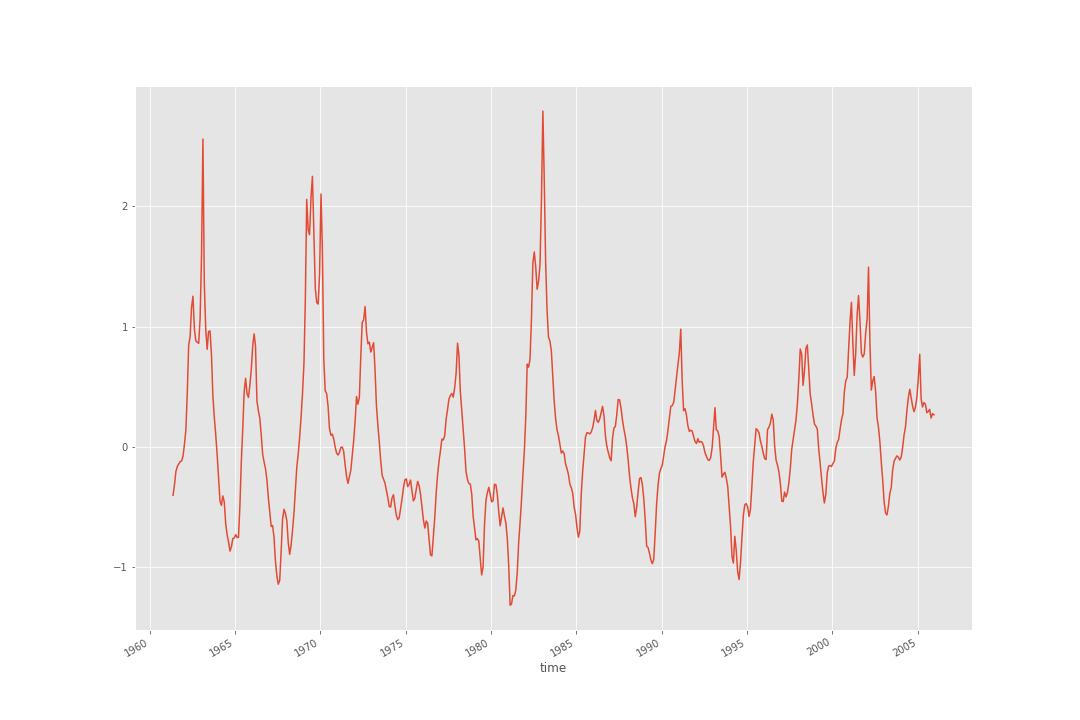
\includegraphics[width=1\textwidth]{gambar24.png}
\end{figure}

\end{document}
